
		\documentclass[a4paper]{article}
		
		%package include
		\usepackage[margin=3cm]{geometry}
		\usepackage[italian]{babel}
		\usepackage[utf8]{inputenc}
		\usepackage[T1]{fontenc}
		\usepackage{graphicx}
		\usepackage{fancyhdr}
		\usepackage{lastpage}
		\usepackage{longtable}
		\usepackage{tabu}
		\usepackage{hyperref}
		\usepackage[hypcap]{caption}
		\usepackage{color}
		\usepackage{xcolor}
		\usepackage{eurosym}
		\usepackage{abstract}
		\usepackage{float}
		\usepackage{listings, lstautogobble}
		\usepackage{amsmath}
		\usepackage{subfigure}
		\usepackage{pifont}
		\usepackage{multirow}

		\colorlet{punct}{red!60!black}
		\definecolor{background}{HTML}{EEEEEE}
		\definecolor{delim}{RGB}{20,105,176}
		\colorlet{numb}{magenta!60!black}


		% per allineare il codice a sinistra invece che al centro
		\lstset{
			autogobble=true,
			escapeinside={(*}{*)}
		}

		\lstdefinelanguage{json}{
		    basicstyle=\normalfont\ttfamily,
		    numbers=left,
		    numberstyle=\scriptsize,
		    stepnumber=1,
		    numbersep=8pt,
		    showstringspaces=false,
		    breaklines=true,
		    frame=lines,
		    backgroundcolor=\color{background},
		    literate=
		     *{0}{{{\color{numb}0}}}{1}
		      {1}{{{\color{numb}1}}}{1}
		      {2}{{{\color{numb}2}}}{1}
		      {3}{{{\color{numb}3}}}{1}
		      {4}{{{\color{numb}4}}}{1}
		      {5}{{{\color{numb}5}}}{1}
		      {6}{{{\color{numb}6}}}{1}
		      {7}{{{\color{numb}7}}}{1}
		      {8}{{{\color{numb}8}}}{1}
		      {9}{{{\color{numb}9}}}{1}
		      {:}{{{\color{punct}{:}}}}{1}
		      {,}{{{\color{punct}{,}}}}{1}
		      {\{}{{{\color{delim}{\{}}}}{1}
		      {\}}{{{\color{delim}{\}}}}}{1}
		      {[}{{{\color{delim}{[}}}}{1}
		      {]}{{{\color{delim}{]}}}}{1},
		}
		

		%macro definitions
		\newcommand{\groupname}{Kaizen Team}
\newcommand{\projectname}{Norris}

\newcommand{\proponente}{Maccagnan Alessandro}
\newcommand{\committente}{Vardanega Tullio}

\newcommand{\insglo}[1]{#1{\ped G}}
\newcommand{\ignoreglo}[1]{#1}
\newcommand{\insdate}[3]{#3-#2-#1}
\newcommand{\instime}[2]{#1-#2}
\newcommand{\insuri}[1]{\textcolor{blue}{\texttt{\url{#1}}}}
\newcommand{\inspath}[1]{\texttt{#1}}
\newcommand{\insrole}[1]{\textit{#1}}
\newcommand{\insdoc}[1]{\textit{“#1”}}
\newcommand{\insfile}[1]{“\texttt{#1}”}
\newcommand{\insrev}[1]{\textbf{#1}}
\newcommand{\insphase}[1]{\textbf{#1}}
\newcommand{\inslabel}[1]{\textit{“#1”}}

		\newcommand{\doctitle}{Specifica Tecnica}
		\newcommand{\lastversion}{5.00}
		

		%abstract font
		\renewcommand{\abstractnamefont}{\huge\bfseries}
		\renewcommand{\abstracttextfont}{\large}

		%hyperred
		\hypersetup{
			linktoc=all,
			colorlinks=true,
			allcolors=black,
			urlcolor=blue,
			bookmarksdepth=100
		}

		%section counters
		\makeatletter
		\newcommand\level[1]{%
			\ifcase#1\relax\expandafter\chapter\or
				\expandafter\section\or
				\expandafter\subsection\or
				\expandafter\subsubsection\else
				\def\next{\@level{#1}}\expandafter\next
			\fi}
		\newcommand{\@level}[1]{%
			\@startsection{level#1}%
				{#1}%
				{\z@}%
				{-3.25ex\@plus -1ex \@minus -.2ex}%
				{1.5ex \@plus .2ex}%
				{\normalfont\normalsize\bfseries}}

		\newdimen\@numsdim
		\newdimen\@dotsdim
		{\normalfont\normalsize
			\sbox\z@{0}\global\@numsdim=\wd\z@
			\sbox\z@{.}\global\@dotsdim=\wd\z@
		}

		\newdimen\@numindent
		\newdimen\@textindent
		\setlength{\@numindent}{15pt}
		\setlength{\@textindent}{15pt}


		\newcounter{level4}[subsubsection]
		\@namedef{thelevel4}{\thesubsubsection.\arabic{level4}}
		\@namedef{level4mark}#1{}
		%\def\l@section{\@dottedtocline{1}{\dimexpr\@numindent*0\relax}{\dimexpr\@dotsdim*0+\@numsdim*1+\@textindent\relax}}
		\def\l@subsection{\@dottedtocline{2}{\dimexpr\@numindent*1\relax}{\dimexpr\@dotsdim*1+\@numsdim*2+\@textindent\relax}}
		\def\l@subsubsection{\@dottedtocline{3}{\dimexpr\@numindent*2\relax}{\dimexpr\@dotsdim*2+\@numsdim*3+\@textindent\relax}}
		\@namedef{l@level4}{\@dottedtocline{4}{\dimexpr\@numindent*3\relax}{\dimexpr\@dotsdim*3+\@numsdim*4+\@textindent\relax}}

		\count@=4
		\def\@ncp#1{\number\numexpr\count@+#1\relax}
		\loop\ifnum\count@<100
			\begingroup\edef\x{\endgroup
				\noexpand\newcounter{level\@ncp{1}}[level\number\count@]
				\noexpand\@namedef{thelevel\@ncp{1}}{%
					\noexpand\@nameuse{thelevel\@ncp{0}}.\noexpand\arabic{level\@ncp{1}}}
				\noexpand\@namedef{level\@ncp{1}mark}####1{}%
				\noexpand\@namedef{l@level\@ncp{1}}%
					{\noexpand\@dottedtocline%
						{\@ncp{1}}%
						{\dimexpr\@numindent*\@ncp{0}\relax}%
						{\the\dimexpr\@dotsdim*\@ncp{0}+\@numsdim*\@ncp{1}+\@textindent\relax}}}%
			\x
			\expandafter\edef\csname toclevel@level\the\count@\endcsname{\the\count@}%
			\advance\count@\@ne
		\repeat
		\makeatother
		
		\setcounter{tocdepth}{100}
		\setcounter{secnumdepth}{100}

		

		%fancyhdr config
		\fancyhf{}
		\fancyhead[L]{
\includegraphics[scale=0.05]{Pics/Logo} 
\includegraphics[height=7mm]{Pics/KaizenTeam}}
		\fancyhead[R]{\Large \bfseries \doctitle \vspace{0.1mm}}

		\fancypagestyle{roman}{
			\hypersetup{linkcolor=black}
			\pagenumbering{Roman}
			\fancyfoot[C]{\thepage{}}
		}

		\fancypagestyle{plain}{
			\hypersetup{linkcolor=blue}
			\pagenumbering{arabic}
			\fancyfoot[C]{\thepage{} di \pageref*{LastPage}}
		}

		
		%space between paragraph
		\raggedbottom
		


		\begin{document}

			\pagestyle{roman}
			\begin{titlepage}
  \begin{center}
	
	
\includegraphics{Pics/KaizenTeam} \\ [1cm]
	
	
\includegraphics[scale=0.6]{Pics/Logo} \\ [1cm]

	
\includegraphics[scale=0.3]{Pics/Norris} \\ [0.5cm]
	
\includegraphics[scale=1]{Pics/CoffeeStrap} \\ [2cm]

	
	\hrule
	\vspace{3mm}
	\Huge{\textbf{\doctitle{} v\lastversion{}}}
	\vspace{3mm}
	\hrule


	\vspace{2cm}

	\begin{minipage}{0.49\textwidth}
		\raggedright \large info@kaizenteam.it
	\end{minipage}
	\begin{minipage}{0.49\textwidth}
		\raggedleft \large \insuri{http://www.kaizenteam.it/}
	\end{minipage}

  \end{center}
\end{titlepage}

			\newpage
			

				\begin{center}
					\tabulinesep=6pt
					\begin{tabu} {X[r]|X[l]}
						\textbf{Versione} & 5.00 \\
						\textbf{Data redazione} & 2015-06-13 \\
						\textbf{Redazione} & \parbox[t]{0.4\textwidth}{Pavanello Fabio Matteo} \\
						\textbf{Verifica} & \parbox[t]{0.4\textwidth}{ Moretto Alessandro \\ Bigarella Chiara} \\
						\textbf{Approvazione} & \parbox[t]{0.4\textwidth}{Carlon Chiara} \\
						\textbf{Uso} & Esterno \\
						\textbf{Distribuzione} & \parbox[t]{0.4\textwidth}{\groupname{} \\ Prof. Vardanega Tullio \\ Prof. Cardin Riccardo \\ CoffeeStrap} \\
					\end{tabu}
				\end{center}

	
			\newpage
			
			\section*{Diario delle modifiche}
				\addtocounter{table}{-1}
				\tabulinesep=3pt
				\begin{longtabu} to \textwidth {|X[c,m]|X[c,m]|X[c,m]|X[c,m]|X[c,m]|}
					\hline
					\rowfont{\bf}
					Versione &
					Data &
					Autore &
					Ruolo &
					Descrizione \\
					\hline
					\endhead
					5.00 &
						2015-06-13 &
						Carlon Chiara &
						Project Manager &
						Approvazione del documento \\
						\hline
					4.04 &
						2015-06-12 &
						Bigarella Chiara &
						Verificatore &
						Verifica incrementi \\
						\hline
					4.03 &
						2015-06-12 &
						Pavanello Fabio Matteo &
						Progettista &
						Fornito maggior dettaglio sulle relazioni individuate tra le componenti \\
						\hline
					4.02 &
						2015-06-11 &
						Moretto Alessandro &
						Verificatore &
						Verifica incrementi \\
						\hline
					4.01 &
						2015-06-10 &
						Pavanello Fabio Matteo &
						Progettista &
						Correzione errori segnalati in RQ \\
						\hline
					4.00 &
						2015-05-27 &
						Pavanello Fabio Matteo &
						Project Manager &
						Approvazione del documento \\
						\hline
					3.16 &
						2015-03-29 &
						Rubin Marco &
						Verificatore &
						Verifica incrementi \\
						\hline
					3.15 &
						2015-05-10 &
						Davide Dal Bianco &
						Verificatore &
						Verifica incrementi \\
						\hline
					3.14 &
						2015-05-10 &
						Bigarella Chiara &
						Progettista &
						Aggiunto paragrafo per spiegare l'utilizzo delle classi factory \\
						\hline
					3.13 &
						2015-05-10 &
						Moretto Alessandro &
						Verificatore &
						Verifica incrementi architettura di Norris e Chuck \\
						\hline
					3.12 &
						2015-05-10 &
						Bucco Riccardo &
						Progettista &
						Lieve modifica architettura Norris e Chuck \\
						\hline
					3.11 &
						2015-05-09 &
						Bucco Riccardo &
						Progettista &
						Spostamento pattern dopo la definizione dell'architettura \\
						\hline
					3.10 &
						2015-05-09 &
						Moretto Alessandro &
						Verificatore &
						Verifica incrementi architettura \\
						\hline
					3.09 &
						2015-05-08 &
						Bigarella Chiara &
						Progettista &
						Correzioni errori rilevati dalla verifica dell'architettura dell'applicazione android \\
						\hline
					3.08 &
						2015-05-08 &
						Moretto Alessandro &
						Verificatore &
						Verifica architettura \\
						\hline
					3.07 &
						2015-05-08 &
						Bigarella Chiara &
						Progettista &
						Modifica architettura dell'applicazione android, da MVC a MVP \\
						\hline
					3.06 &
						2015-05-08 &
						Pavanello Fabio Matteo &
						Verificatore &
						Verifica incrementi \\
						\hline
					3.05 &
						2015-05-08 &
						Carlon Chiara &
						Progettista &
						Approfondita descrizione pattern Bridge \\
						\hline
					3.04 &
						2015-05-08 &
						Bigarella Chiara &
						Progettista &
						Correzione piccoli errori segnalati in RP \\
						\hline
					3.03 &
						2015-05-07 &
						Dal Bianco Davide &
						Verificatore &
						Verifica incrementi \\
						\hline
					3.02 &
						2015-05-07 &
						Carlon Chiara &
						Amministratore &
						Aggiunti svantaggi tecnologie \\
						\hline
					3.01 &
						2015-05-07 &
						Bucco Riccardo &
						Progettista &
						Modificati riferimenti informativi \\
						\hline
					3.00 &
						2015-05-03 &
						Bigarella Chiara &
						Project Manager &
						Approvazione del documento \\
						\hline
					2.02 &
						2015-04-24 &
						Bucco Riccardo &
						Verificatore &
						Verifica modifiche Chuck \\
						\hline
					2.01 &
						2015-04-04 &
						Rubin Marco &
						Progettista &
						Apporto di piccole modifiche architettura Chuck \\
						\hline
					2.00 &
						2015-04-20 &
						Dal Bianco Davide &
						Project Manager &
						Approvazione del documento \\
						\hline
					1.02 &
						2015-04-06 &
						Moretto Alessandro &
						Verificatore &
						Verifica incremento \\
						\hline
					1.01 &
						2015-04-04 &
						Rubin Marco &
						Progettista &
						Apporto di piccole modifiche architetturale Norris \\
						\hline
					1.00 &
						2015-03-31 &
						Rubin Marco &
						Project Manager &
						Approvazione del documento \\
						\hline
					0.16 &
						2015-03-31 &
						Pavanello Fabio Matteo &
						Verificatore &
						Verifica documento \\
						\hline
					0.15 &
						2015-03-29 &
						Bucco Riccardo &
						Progettista &
						Stesura ed importazione tracciamento \\
						\hline
					0.14 &
						2015-03-29 &
						Dal Bianco Davide &
						Project Manager &
						Stesura stime di fattibilità e di bisogno di risorse \\
						\hline
					0.13 &
						2015-03-27 &
						Carlon Chiara &
						Verificatore &
						Verifica componenti applicazione Android \\
						\hline
					0.12 &
						2015-03-26 &
						Pavanello Fabio Matteo &
						Verificatore &
						Verifica componenti Chuck \\
						\hline
					0.11 &
						2015-03-26 &
						Carlon Chiara &
						Verificatore &
						Verifica sezione Dashboard \\
						\hline
					0.10 &
						2015-03-26 &
						Bucco Riccardo &
						Progettista &
						Stesura sezione mockup Dashboard \\
						\hline
					0.09 &
						2015-03-26 &
						Carlon Chiara &
						Verificatore &
						Verifica componenti Norris \\
						\hline
					0.08 &
						2015-03-24 &
						Moretto Alessandro &
						Progettista &
						Stesura e descrizione componenti applicazione Android \\
						\hline
					0.07 &
						2015-03-24 &
						Bucco Riccardo &
						Progettista &
						Stesura e descrizione componenti Chuck \\
						\hline
					0.06 &
						2015-03-23 &
						Dal Bianco Davide &
						Progettista &
						Stesura e descrizione componenti Norris \\
						\hline
					0.05 &
						2015-03-15 &
						Pavanello Fabio Matteo &
						Verificatore &
						Verifica architettura \\
						\hline
					0.04 &
						2015-03-12 &
						Bigarella Chiara &
						Progettista &
						Stesura architettura generale \\
						\hline
					0.03 &
						2015-03-07 &
						Carlon Chiara &
						Verificatore &
						Verifica documento \\
						\hline
					0.02 &
						2015-03-06 &
						Moretto Alessandro &
						Progettista &
						Stesura tecnologie utilizzate \\
						\hline
					0.01 &
						2015-03-05 &
						Bigarella Chiara &
						Progettista &
						Struttura ed introduzione del documento \\
						\hline
					
				\end{longtabu}

	
			\newpage

			
			\tableofcontents
			\newpage
			\listoftables
			\newpage
			\listoffigures
			\newpage
			\pagestyle{plain}

			
		\newpage
		\level{1}{Introduzione}
	\level{2}{Scopo del documento}
		Il presente documento intende stabilire le varie norme che il gruppo \groupname{} segue nello sviluppo del progetto \projectname{}. Esso, inoltre, indica gli strumenti e le procedure da utilizzare. Infine, vengono descritte le attività che il gruppo deve affrontare durante lo sviluppo.\\
		Ciascun componente è obbligato a prendere visione di tale documento e a rispettare le norme in esso descritte. Qualora nel documento fossero presenti delle convenzioni, non è strettamente obbligatorio seguirle, sebbene sia caldamente consigliato.\\
		Tutti i contenuti di tale documento permettono di migliorare l’efficienza del lavoro svolto. Essi, inoltre, servono a facilitare la \insglo{fase} di verifica e a garantire una maggiore coerenza tra i documenti prodotti.\\
		Segue un riassunto di quanto contenuto all'interno di tale documento:
		\begin{itemize}
			\item organizzazione della comunicazione tra i vari membri del \insglo{team};
			\item metodologia di stesura dei documenti;
			\item descrizione del modo in cui il lavoro viene organizzato durante lo sviluppo del progetto;
			\item strumenti utilizzati per gestire l'ambiente di lavoro, il \insglo{repository} ed il \textit{ticketing}.
		\end{itemize}

	\subsection{Glossario}
	Allo scopo di rendere più semplice la comprensione dei documenti ed evitare eventuali ambiguità, viene allegato il \insdoc{Glossario v1.00}, che contiene la spiegazione della terminologia tecnica e degli acronimi utilizzati. Per facilitare la lettura, i termini presenti all'interno di tale documento saranno marcati da una “G” maiuscola a pedice.
	

	\level{2}{Riferimenti utili}
		\level{3}{Riferimenti normativi}
			\begin{itemize}
				\item\textbf{\insglo{Capitolato} d'appalto C3:} \projectname{}: Real-time Business Intelligence \\
					\insuri{http://www.math.unipd.it/~tullio/IS-1/2014/Progetto/C3.pdf}.
			\end{itemize}
		\level{3}{Riferimenti informativi}
			\begin{itemize}
				\item \textbf{Materiale del corso di Ingegneria del \insglo{Software}:} \\
					\insuri{http://www.math.unipd.it/~tullio/IS-1/2014/Dispense/P05.pdf};\\
					\insuri{http://www.math.unipd.it/~tullio/IS-1/2014/Dispense/P06.pdf}; \\
					\insuri{http://www.math.unipd.it/~tullio/IS-1/2014/Dispense/P12.pdf};
				\item \textbf{\insglo{Git}:} \insuri{http://git-scm.com/};
				\item \textbf{Portable Document Format:} \\
					\insuri{http://en.wikipedia.org/wiki/Portable\_Document\_Format};
				\item \textbf{Portable Network Graphics:} \\
					\insuri{http://en.wikipedia.org/wiki/Portable\_Network\_Graphics};
				\item \textbf{Unicode:} \insuri{http://en.wikipedia.org/wiki/Unicode}.
			\end{itemize}

	
		\newpage
		\level{1}{Tecnologie utilizzate}
In questa sezione sono elencate le principali tecnologie utilizzate per lo sviluppo del progetto. Per ognuna di esse viene descritto lo scopo per il quale vengono usate ed i vantaggi che se ne ricavano.
\level{2}{Node.js}
\level{3}{Descrizione}
L'utilizzo di \insglo{Node.js} è stato richiesto dal proponente. Si tratta di un sistema run-time cross-platform che utilizza l'engine Google V8 \insglo{JavaScript} per eseguire il codice; viene utilizzato nello sviluppo di applicazioni real-time, lato \insglo{server} e di rete. Nel progetto viene usato per la realizzazione della libreria come piattaforma di sviluppo.
\level{3}{Vantaggi}
I vantaggi nell'utilizzo di \insglo{Node.js} sono i seguenti:
\begin{itemize}
\item fornisce una semplice soluzione per lo sviluppo di programmi scalabili;
\item essendo leggero ed efficiente è particolarmente indicato per applicazioni real-time con un intensivo uso di dati;
\item usa un sistema I/O asincrono, non bloccante, basato su eventi; questo permette di sviluppare più facilmente sistemi responsivi.
\end{itemize}
\level{3}{Svantaggi}
Seguono gli svantaggi rilevati nell'utilizzo di \insglo{Node.js}:
\begin{itemize}
	\item essendo un linguaggio di recente creazione, alcuni moduli risultano instabili;
	\item essendo un linguaggio single-threaded, non è performante in caso di applicazioni con uso intensivo di CPU;
	\item utilizzando un sistema I/O asincrono, è possibile che l'uso di \insglo{callback} risulti eccessivo.
\end{itemize}

\level{2}{Socket.io}
\level{3}{Descrizione}
L'uso di \insglo{Socket.io} è stato richiesto dal proponente. È una libreria \insglo{JavaScript} che permette comunicazioni real-time bidirezionali e basate su eventi. Viene utilizzato per implementare la trasmissione degli aggiornamenti dei grafici.
\level{3}{Vantaggi}
L'utilizzo di \insglo{Socket.io} fornisce i seguenti vantaggi:
\begin{itemize}
\item permette di creare comunicazioni bi-direzionali tra \insglo{client} e \insglo{server};
\item gestisce la connessione in modo trasparente;
\item ogniqualvolta il \insglo{browser} lo supporti usa il protocollo \insglo{WebSocket}, il quale fornisce canali di comunicazione bidirezionali simultanei attraverso una singola connessione \insglo{TCP}.
\end{itemize}
\level{3}{Svantaggi}
L'utilizzo di \insglo{Socket.io} porta, anche, ad alcuni svantaggi:
\begin{itemize}
	\item richiede che, sia \insglo{client} che \insglo{server}, utilizzino le librerie di \insglo{Socket.io};
	\item essendo una tecnologia di recente creazione, soffre ancora di alcuni bug.
\end{itemize}

\level{2}{Express.js}
\level{3}{Descrizione}
\insglo{Express.js} è un \insglo{framework} di \insglo{Node.js} che mette a disposizione un \insglo{middleware} utilizzabile per la realizzazione dell'infrastruttura web. Il suo utilizzo è stato richiesto dal proponente.
\level{3}{Vantaggi}
\insglo{Express.js} permette di estendere il modulo \texttt{\insglo{http}} di \insglo{Node.js} rendendo più facile la gestione dell'indirizzamento del \insglo{server}, delle risposte, dei cookie e delle richieste di stato \insglo{HTTP}.
\level{3}{Svantaggi}
Non sono stati rilevati grossi svantaggi nell'uso di \insglo{Express.js}, il quale risulta essere un buon \insglo{framework} che fornisce molti metodi per estendere il modulo \insglo{http} di \insglo{Node.js}.

\level{2}{HTML5}
\level{3}{Descrizione}
Si è scelto di utilizzare HTML5 come \insglo{linguaggio di markup} per la creazione delle pagine web.
\level{3}{Vantaggi}
I vantaggi dell'uso di HTML5 sono i seguenti:
\begin{itemize}
\item è il linguaggio utilizzato dalla libreria \insglo{Chart.js} per produrre i grafici;
\item HTML5 è supportato da tutti i più recenti \insglo{browser};
\item assieme a CSS permette di creare pagine web più interattive;
\item è stato decretato standard dal W3C.
\end{itemize}
\level{3}{Svantaggi}
Nell'uso di HTML5, sono stati rilevati i seguenti svantaggi:
\begin{itemize}
\item è supportato solo dalle versioni più recenti dei \insglo{browser};
\item è un linguaggio ancora in via di sviluppo, il che comporta un possibile cambiamento dei costrutti; tuttavia la maggior parte di questo linguaggio è stata considerata stabile.
\end{itemize}

\level{2}{CSS3}
\level{3}{Descrizione}
È stato scelto di usare CSS3 come linguaggio di formattazione dei documenti HTML. Grazie ad esso è possibile fornire un \insglo{layout} alle pagine web per renderle accessibili ed usabili.
\level{3}{Vantaggi}
I vantaggi dell'uso di CSS3 sono i seguenti:
\begin{itemize}
\item permette il riuso del codice, il che comporta una maggiore velocità di caricamento delle pagine web;
\item consente una manutenzione più semplice e veloce;
\item permette la separazione tra la struttura e la presentazione.
\end{itemize}
\level{3}{Svantaggi}
L'unico svantaggio rilevato dall'uso di CSS3 è dato dal fatto che, essendo un linguaggio ancora in via di sviluppo, è supportato (non appieno) solo dai web \insglo{browser} più recenti.

\level{2}{AngularJS}
\level{3}{Descrizione}
AngularJS è un \insglo{framework} \insglo{MVC} \insglo{JavaScript} che fornisce un metodo ben strutturato per la creazione di siti e applicazioni web. Questo \insglo{framework} è la libreria lato \insglo{client} ideale da usare insieme a \insglo{Node.js}.
\level{3}{Vantaggi}
L'utilizzo di AngularJS fornisce i seguenti vantaggi:
\begin{itemize}
\item fornisce un approccio pulito e strutturato per la creazione delle applicazioni lato \insglo{client};
\item utilizza gli oggetti \insglo{JavaScript};
\item facilita la corretta implementazione del \insglo{pattern} \insglo{MVC};
\item fornisce una semplice e flessibile interfaccia di filtraggio che permette di filtrare i dati nel passaggio da Model a View.
\end{itemize}
\level{3}{Svantaggi}
Uno degli svantaggi rilevato nell'uso di \insglo{Angular.js} è la documentazione povera di esempi d'utilizzo. Tuttavia, questo può essere risolto tramite un'approfondita ricerca nel web. Un altro svantaggio deriva dal fatto che il codice non è valido secondo lo standard del W3C. 

\level{2}{Chart.js}
\level{3}{Descrizione}
È stato scelto di usare la libreria \insglo{JavaScript} \insglo{Chart.js} per la creazione di grafici in HTML5.
\level{3}{Vantaggi}
I vantaggi dell'uso di \insglo{Chart.js} sono i seguenti:
\begin{itemize}
\item usa l'elemento canvas di HTML5, il quale è supportato da tutti i \insglo{browser} più recenti;
\item è libero da dipendenze ed è leggero;
\item fornisce un sistema responsive (ad esempio i grafici vengono ridimensionati se la finestra del \insglo{browser} cambia dimensioni);
\item essendo modulare, permette di caricare solo i grafici di cui si ha bisogno.
\end{itemize}
\level{3}{Svantaggi}
Non sono stati riscontrati grossi svantaggi nell'uso di tale libreria, la quale è accompagnata da una documentazione organizzata e ben fornita, anche, di numerosi esempi.

\level{2}{DataTables}
\level{3}{Descrizione}
È stato scelto di usare la libreria \insglo{JavaScript} \insglo{DataTables} per la creazione di tabelle in HTML5. Tale libreria permette la creazione di tabelle dinamiche ed interattive. \insglo{DataTables} fornisce delle \insglo{API} per la manipolazione delle tabelle e per l'accesso ai dati contenuti in esse. 
\level{3}{Vantaggi}
L'utilizzo di \insglo{DataTables} offre i seguenti vantaggi:
\begin{itemize}
\item fornisce numerose opzioni aggiuntive ed estensioni, che rendono ampiamente personalizzabili le tabelle create;
\item fornisce metodi di ordinamento dei dati, che possono essere personalizzati a seconda delle necessità;
\item permette il filtraggio dei dati, basato sui dati o sulle righe;
\item permette la personalizzazione delle opzioni di impaginamento delle tabelle, in modo che siano facili da consultare per l'utente finale.
\end{itemize}
\level{3}{Svantaggi}
Nell'uso di \insglo{DataTables} non sono stati rilevati grossi svantaggi. \insglo{DataTables} offre un'ampia documentazione piena di esempi d'uso. Inoltre, grazie al forum, presente sul sito web ufficiale, si possono ottenere risposte ad eventuali problemi o dubbi che sorgono durante l'utilizzo della libreria.

\level{2}{OpenStreetMap}
\level{3}{Descrizione}
È stato scelto di utilizzare OpenStreetMap, per la visualizzazione di Map Charts, un progetto collaborativo finalizzato alla creazione di dati cartografici, liberi e gratuiti a chiunque. Il progetto è stato lanciato poiché molte delle mappe che normalmente si pensano libere, hanno in realtà restrizioni legali o tecniche. OpenStreetMap mette, inoltre, a disposizione i geodati su cui le mappe si basano, al contrario di moltre altre librerie, come Google Maps \insglo{API}.
\level{3}{Vantaggi}
L'utilizzo di OpenStreetMap offre i seguenti vantaggi:
\begin{itemize}
\item libertà: i dati geografici e le mappe di OpenStreetMap sono rilasciati con licenza creata specificamente per proteggere i \insglo{database}, la quale permette la copia, la modifica e la ridistribuzione delle mappe, inoltre sono completamente gratuite, quindi non occorre pagare per usufruire di funzionalità aggiuntive;
\item affidabilità: le mappe sono prive di errori inseriti volutamente per riconoscere le mappe copiate;
\item copertura mondiale: essendo un progetto collaborativo a livello mondiale, offre mappe molto precise di tutto il mondo;
\item flessibilità: i dati di OpenStreetMap possono essere usati in molte maniere diverse, principalmente per creare mappe ma anche per copiarle, trasferirle e modificarle per qualsiasi scopo.
\end{itemize}
\level{3}{Svantaggi}
Gli unici svantaggi, derivanti dall'uso di OpenStreetMap, sono inerenti alla precisione delle mappe, i cui dati non essendo controllati sistematicamente, possono mancare di precisione ed accuratezza.

\level{2}{MPAndroidChart}
\level{3}{Descrizione}
Si è scelto di utilizzare MPAndroidChart, una libreria per la creazione di chart in \insglo{Android}. Essa viene usata per la creazione di \insglo{bar chart} e \insglo{line chart}, ma ne supporta molti altri come pie chart, radar chart e scatter chart. Tale libreria fornisce anche delle funzioni di scaling (ridimensionamento), dragging (trascinamento), selecting (selezione) e di animazione. La scelta di una libreria per la creazione di chart in \insglo{Android} è ricaduta su MPAndroidChart principalmente per le poche librerie a disposizione, tuttavia sono comunque stati trovati alcuni aspetti positivi.
\level{3}{Vantaggi}
MPAndroidChart fornisce i seguenti benefici:
\begin{itemize}
\item ridimensionamento su entrambi gli assi di un chart, tramite touch-\insglo{gesture}, in modo separato;
\item salvataggio dei chart su SD-Card come immagini;
\item template di impostazioni predefinite;
\item legende create automaticamente ma personalizzabili;
\item grafici ampiamente personalizzabili.
\end{itemize}
\level{3}{Svantaggi}
Non sono stati trovati svantaggi nell'uso di tale libreria. Essa è accompagnata da un'ampia documentazione, che ci ha permesso uno studio più rapido e più semplice grazie ai numerosi esempi forniti.

\level{2}{GoogleMaps Android API v2}
\level{3}{Descrizione}
Si è scelto di utilizzare GoogleMaps \insglo{Android} \insglo{API} v2 per la visualizzazione di mappe. Tale libreria permette di aggiungere mappe basate sui dati di Google Maps, alla propria applicazione. Le \insglo{API} gestiscono automaticamente l'accesso ai \insglo{server} di Google Maps, il download dei dati, la visualizzazione della mappa e le risposte alle \insglo{gesture}. Inoltre è possibile usare tali \insglo{API} per aggiungere markers e per cambiare la view di una particolare area di una mappa.
\level{3}{Vantaggi}
L'utilizzo di GoogleMaps \insglo{Android} \insglo{API} v2 fornisce i seguenti vantaggi:
\begin{itemize}
\item è possibile inserire una mappa in un'\insglo{activity} come un fragment, con un semplice frammento di codice \insglo{XML};
\item fornisce nuove funzionalità come: mappe 3D, satellite, terreno, mappe ibride e transizioni animate
\item offre la possibilità di aggiungere la visualizzazione “StreetView”.
\end{itemize}
\level{3}{Svantaggi}
Non sono stati riscontrati grossi svantaggi nell'uso di tale libreria, la quale è accompagnata da una documentazione ben organizzata. Inoltre, si possono trovare facilmente online, molti esempi e tutorial.

	
		\newpage
		\level{1}{Descrizione generale dei prodotti}
    Riportiamo di seguito una descrizione generale dei prodotti. Per una descrizione più dettagliata delle funzionalità dei prodotti, si rimanda al documento \insdoc{Analisi dei Requisiti 3.00}.

    \level{2}{Norris}
    Norris è un framework per Node.js che permette di raccogliere dati provenienti da sorgenti arbitrarie e visualizzarli come grafici in modo semplice e veloce. In particolare mette a disposizione dei suoi utenti due interfacce:
    \begin{itemize}
        \item le API interne (lato server);
        \item le API esterne (lato client).
    \end{itemize}
    
    \level{3}{API interne}
    Tramite le API interne, uno sviluppatore può creare lato server un'istanza di Norris. Può, inoltre, creare quattro tipologie di grafici: bar chart, line chart, map chart e table. Per ogni grafico può configurare le relative impostazioni e può impostare il metodo di aggiornamento dei dati del grafico stesso. L'aggiornamento dei grafici può essere di tre tipologie, a seconda del tipo di grafico:
    \begin{itemize}
        \item in place, supportato da tutti i tipi di chart;
        \item stream, supportato da bar chart, line chart e table;
        \item movie, supportato da map chart.
    \end{itemize}
    
    
    
    Lo sviluppatore può, inoltre, scegliere di incapsulare alcuni grafici all'interno di una o più pagine web. Le API interne permettono infatti di aggiungere i grafici creati ad una o più pagine web, le quali verrano create in automatico da Norris. Lo sviluppatore, oltre a poter scegliere quali grafici inserire in queste pagine, può configurare le impostazioni di ciascuna di esse. Tra le impostazioni principali ci sono la scelta del titolo e del template della pagina.\\
    Infine, se lo sviluppatore non vuole rendere pubblici i propri grafici, può definire una funzione login, una funzione islogged e una funzione di logout. Queste verranno eseguite ogni qualvolta venga richiesto di accedere alle informazioni di un grafico.
   
   \level{3}{API esterne}
   Tramite le API esterne, un utente lato client può effettuare l'autenticazione ad un'istanza di Norris esistente e richiedere al server le informazioni inerenti ai grafici presenti in quell'istanza. In particolare l'utente client può richiedere la lista dei grafici presenti nell'istanza, nonchè le informazioni di ogni singolo grafico della lista. Le informazioni verranno fornite in formato JSON.

    \level{2}{Chuck}
    Chuck, acronimo di Chart Universal Creator Kit, è una libreria Javascript lato client che permette di incapsulare un grafico (creato tramite le API interne di Norris) all'interno di una pagina web diversa da quelle create di default da Norris. In particolare lo sviluppatore lato client deve autenticarsi ad un'istanza di Norris, richiedere un grafico e scegliere il tag HTML in cui inserire il grafico. È possibile, inoltre, modificare alcune impostazioni relative al grafico.
    
   \level{2}{Applicazione Android}
    L'applicazione Android permette di visualizzare i grafici di un'istanza di Norris da uno smartphone Android. Essa permette di scegliere l'istanza di Norris alla quale connettersi tramite autenticazione. Una volta autenticato, l'utente può visualizzare la lista di grafici esistenti e i grafici stessi.
        
\level{1}{Descrizione delle interazioni che i prodotti hanno tra di loro}
     \level{2}{Norris - Chuck}
    Norris e Chuck interagiscono tramite le API esterne, le quali fungono da interfaccia tra server e client. In particolare si possono avere 3 tipologie di interazione:
    \begin{itemize}
        \item autenticazione: precede l'invio di informazioni inerenti un grafico. Chuck manda a Norris l'indirizzo dell'istanza a cui si vuole connettere, assieme ad username e password. Norris controlla se i dati inviati sono corretti e, in caso affermativo, esegue l'autenticazione.
        \item richiesta inserimento grafico: Chuck manda a Norris una richiesta di informazioni inerenti al grafico che si vuole inserire nella pagina web. Norris controlla se il client è autenticato. In caso negativo, Norris manda una richiesta di autenticazione al client. In caso affermativo, invece, Norris manda le informazioni relative al grafico richiesto aprendo una comunicazione tramite websocket. Il canale rimane aperto fintanto che il client rimane connesso.
        \item aggiornamenti del grafico: quando un grafico viene aggiornato lato server, Norris si preoccupa di mandare l'aggiornamento ai client che hanno quel grafico. La comunicazione dell'aggiornamento avviene tramite un canale websocket appositamente creato al momento della richiesta di inserimento del grafico nella pagina web.
    \end{itemize}
    
    \level{2}{Norris - Applicazione Android}
    Norris e l'applicazione Android interagiscono tramite le API esterne, le quali fungono da interfaccia tra server e client. In particolare si possono avere 4 tipologie di interazione:
    \begin{itemize}
        \item Autenticazione: precede l'invio di informazioni inerenti un grafico. L'applicazione Android manda a Norris l'indirizzo dell'istanza a cui si vuole connettere, assieme ad username e password. Norris controlla se i dati inviati sono corretti e, in caso affermativo, esegue l'autenticazione. Se l'autenticazione non va a buon fine, l'applicazione Android mostra un messaggio d'errore.
        \item Richiesta informazioni della lista di grafici: l'applicazione Android manda a Norris una richiesta di informazioni inerenti alla lista di grafici presenti nell'istanza di Norris alla quale ci si è autenticati. Norris controlla se l'utente è loggato e, in caso affermativo, manda le informazioni relative alla lista di grafici richiesta aprendo una comunicazione tramite websocket. Il canale viene chiuso quando l'applicazione è in background.
        \item Richiesta informazioni di un grafico: l'applicazione Android manda a Norris una richiesta di informazioni inerenti al grafico che si vuole inserire nella pagina web. Norris controlla se il client è autenticato e, in caso affermativo, manda le informazioni relative al grafico richiesto aprendo una comunicazione tramite websocket. Il canale viene chiuso quando il grafico o l'applicazione sono in background.
        \item Aggiornamenti del grafico: quando un grafico viene aggiornato lato server, Norris si preoccupa di mandare l'aggiornamento ai client che hanno quel grafico. La comunicazione dell'aggiornamento avviene tramite un canale websocket appositamente creato al momento dell'invio dell'aggiornamento. Il canale viene chiuso quando il grafico o l'applicazione sono in background. Gli aggiornamenti avranno luogo solo quando il grafico è attivo. Se il grafico è in background, gli aggiornamenti vengono ignorati.
    \end{itemize}

	
		\newpage
		\level{1}{Progettazione architetturale dei prodotti}
	\level{1}{Norris}
    \level{2}{Specifica dei componenti}
	Nella presente sezione è stata riportata e documentata la progettazione di dettaglio del \insglo{prodotto} \insglo{Norris}. Si noti che tale progettazione deriva direttamente dalla progettazione architetturale che può essere trovata all'interno del documento \insdoc{Specifica Tecnica v4.00}. I risultati ottenuti sono stati organizzati e presentati secondo la seguente struttura:
	\begin{enumerate}
		\item vengono innanzitutto presentate le varie classi che sono state individuate. Per ognuna di esse si indica il nome, il tipo, l'eventuale astrattezza, la visibilità e il fatto che estenda altre classi oppure no. In aggiunta a ciò, viene presentata una descrizione completa del ruolo e delle responsabilità della classe oltre a una documentazione completa riguardante tutti gli attributi e i metodi presenti all'interno.
		\item in secondo luogo vengono presentati i diagrammi di sequenza, che hanno lo scopo di descrivere scenari (determinate sequenze di azioni in cui tutte le scelte sono già state effettuate). Essi vengono usati per descrivere le relazioni che intercorrono, in termini di messaggi, tra attori, oggetti ed entità del sistema \insglo{Norris}.
	\end{enumerate}
	Le regole che sono state rispettate, gli strumenti che sono stati usati e le procedure che sono state effettuate possono essere trovate all'interno del documento \insdoc{Norme di Progetto v6.00}.
    \level{3}{Classi}
    	In tale sezione sono riportate delle descrizioni dettagliate delle classi individuate all'interno del documento \insdoc{Specifica Tecnica v4.00}. Tali classi sono presentate e organizzate in modo gerarchico, mantenendo una suddivisione per \insglo{package} di appartenenza.
        \level{1}{Norris}
    \level{2}{Specifica dei componenti}
	Nella presente sezione è stata riportata e documentata la progettazione di dettaglio del \insglo{prodotto} \insglo{Norris}. Si noti che tale progettazione deriva direttamente dalla progettazione architetturale che può essere trovata all'interno del documento \insdoc{Specifica Tecnica v4.00}. I risultati ottenuti sono stati organizzati e presentati secondo la seguente struttura:
	\begin{enumerate}
		\item vengono innanzitutto presentate le varie classi che sono state individuate. Per ognuna di esse si indica il nome, il tipo, l'eventuale astrattezza, la visibilità e il fatto che estenda altre classi oppure no. In aggiunta a ciò, viene presentata una descrizione completa del ruolo e delle responsabilità della classe oltre a una documentazione completa riguardante tutti gli attributi e i metodi presenti all'interno.
		\item in secondo luogo vengono presentati i diagrammi di sequenza, che hanno lo scopo di descrivere scenari (determinate sequenze di azioni in cui tutte le scelte sono già state effettuate). Essi vengono usati per descrivere le relazioni che intercorrono, in termini di messaggi, tra attori, oggetti ed entità del sistema \insglo{Norris}.
	\end{enumerate}
	Le regole che sono state rispettate, gli strumenti che sono stati usati e le procedure che sono state effettuate possono essere trovate all'interno del documento \insdoc{Norme di Progetto v6.00}.
    \level{3}{Classi}
    	In tale sezione sono riportate delle descrizioni dettagliate delle classi individuate all'interno del documento \insdoc{Specifica Tecnica v4.00}. Tali classi sono presentate e organizzate in modo gerarchico, mantenendo una suddivisione per \insglo{package} di appartenenza.
        \input{Classi/Norris.tex}

    \level{3}{Classi aggiuntive}
        Per quanto riguarda le classi aggiuntive riguardanti che implementano i tipi “ChartSettings” e “ChartUpdate” si faccia riferimento all'appendice \nameref{app:schemi}, nella quale sono presenti gli schemi \insglo{JSON} di tali oggetti.
        \input{Classi/NorrisAggiuntive.tex}

    \level{2}{Diagrammi di sequenza}
    	In tale sezione vengono presentati i diagrammi di sequenza, che hanno lo scopo di descrivere scenari (determinate sequenze di azioni in cui tutte le scelte sono già state effettuate). Essi vengono usati per descrivere le relazioni che intercorrono, in termini di messaggi, tra attori, oggetti ed entità del sistema \insglo{Norris}.
        \level{3}{Creazione di un chart}
        	Tale diagramma descrive come viene creato un chart di un certo tipo prefissato.
            \begin{figure}[H]
                \centering
                \includegraphics[scale=0.3]{DefinizioneDiProdotto/Pics/NorrisCreazioneChart}
                \caption{Diagramma di sequenza - Norris, creazione chart}
            \end{figure}


        \level{3}{Aggiornamento di un chart}
        	Tale diagramma descrive come viene aggiornato un chart di un certo tipo (sulla base delle modalità di aggiornamento definite per quel tipo di grafico).
            \begin{figure}[H]
                \centering
                \includegraphics[scale=0.3]{DefinizioneDiProdotto/Pics/NorrisAggiornamentoChart}
                \caption{Diagramma di sequenza - Norris, aggiornamento chart}
            \end{figure}

            
        \level{3}{Invio lista dei grafici}
        	Tale diagramma descrive come viene gestita la richiesta della lista di tutti i grafici contenuti in una certa istanza di \insglo{Norris}.
            \begin{figure}[H]
                \centering
                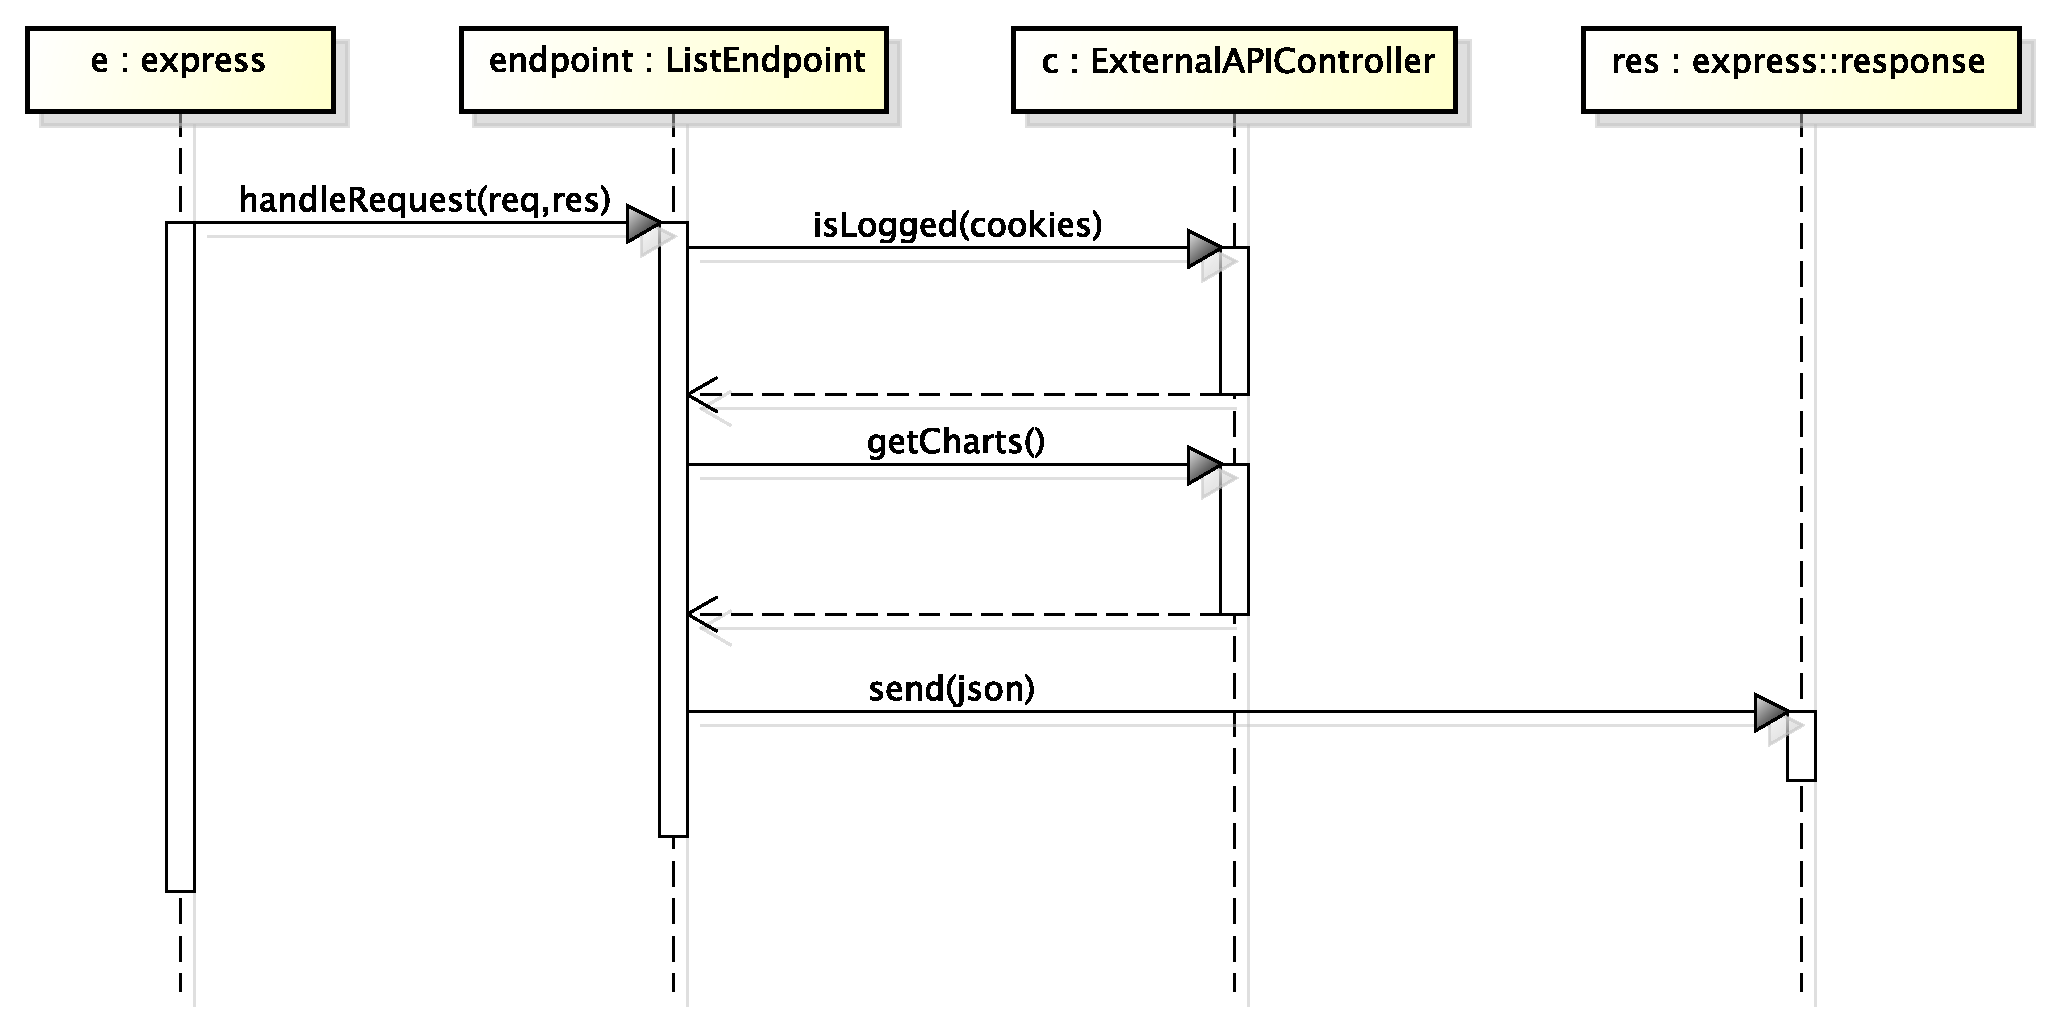
\includegraphics[scale=0.3]{DefinizioneDiProdotto/Pics/NorrisInvioLista}
                \caption{Diagramma di sequenza - Norris, invio lista}
            \end{figure}

            
        \level{3}{Invio di un chart}
        	Tale diagramma descrive come viene gestita la richiesta di un chart da parte di un \insglo{client} dal sistema \insglo{Norris}.
            \begin{figure}[H]
                \centering
                \includegraphics[scale=0.3]{DefinizioneDiProdotto/Pics/NorrisInvioChart}
                \caption{Diagramma di sequenza - Norris, invio chart}
            \end{figure}


    \level{3}{Classi aggiuntive}
        Per quanto riguarda le classi aggiuntive riguardanti che implementano i tipi “ChartSettings” e “ChartUpdate” si faccia riferimento all'appendice \nameref{app:schemi}, nella quale sono presenti gli schemi \insglo{JSON} di tali oggetti.
        
			\level{4}[NorrisSettingsImpl]{NorrisAggiuntive::NorrisSettingsImpl}
			

		\IfFileExists{DefinizioneDiProdotto/Pics/ClassiAggiuntive/NorrisSettingsImpl.pdf}{
			\begin{figure}[H]
				\centering
				\includegraphics[scale=0.5]{DefinizioneDiProdotto/Pics/ClassiAggiuntive/NorrisSettingsImpl}
				\caption{NorrisSettingsImpl}
			\end{figure}
		}
	
			
			\begin{itemize}
			\item \textbf{Nome:} NorrisSettingsImpl
			\item \textbf{Tipo:} classe
			
		\item \textbf{Astratta:}
		no
			\item \textbf{Visibilità:} public
			\item \textbf{Descrizione:} La classe NorrisSettingsImpl definisce le impostazioni relative ad un'istanza di Norris. Lo sviluppatore può definire le funzioni che verranno eseguite per l'autenticazione.
			\item \textbf{Attributi:}
				\begin{itemize}
				\setlength{\itemsep}{5pt}
				
					\item[\ding{111}] {+login : Function} \\ [1mm] L'attributo login rappresenta la funzione che verrà eseguita per avviare la sessione di un utente.
					\item[\ding{111}] {+logout : Function} \\ [1mm] L'attributo login rappresenta la funzione che verrà eseguita per terminare la sessione di un utente.
					\item[\ding{111}] {+keepAlive : Function} \\ [1mm] L'attributo login rappresenta la funzione che verrà eseguita per rinnovare la sessione di un utente.
					\item[\ding{111}] {+isLogged : Function} \\ [1mm] L'attributo login rappresenta la funzione che verrà eseguita per verificare lo stato dela sessione di un utente.
					\item[\ding{111}] {+endpoint : String} \\ [1mm] L'attributo endpoint definisce il path al quale sono disponibili le API esterne.
					\item[\ding{111}] {+secret : String} \\ [1mm] L'attributo secret definisce la chiave di cifrature per i cookie firmati.
					\item[\ding{111}] {+origins : String[]} \\ [1mm] L'attributo origin definisce gli host attendibili, verso i quali saranno disponibili le API esterne.
				\end{itemize}
		
			\end{itemize}
	
			\level{4}[PageSettingsImpl]{NorrisAggiuntive::PageSettingsImpl}
			

		\IfFileExists{DefinizioneDiProdotto/Pics/ClassiAggiuntive/PageSettingsImpl.pdf}{
			\begin{figure}[H]
				\centering
				\includegraphics[scale=0.5]{DefinizioneDiProdotto/Pics/ClassiAggiuntive/PageSettingsImpl}
				\caption{PageSettingsImpl}
			\end{figure}
		}
	
			
			\begin{itemize}
			\item \textbf{Nome:} PageSettingsImpl
			\item \textbf{Tipo:} classe
			
		\item \textbf{Astratta:}
		no
			\item \textbf{Visibilità:} public
			\item \textbf{Descrizione:} La classe PageSettingsImpl definisce le impostazioni di una pagina di Norris.
			\item \textbf{Attributi:}
				\begin{itemize}
				\setlength{\itemsep}{5pt}
				
					\item[\ding{111}] {+title : String} \\ [1mm] L'attributo title rappresenta il titolo di una pagina di Norris.
					\item[\ding{111}] {+maxChartsRow : int} \\ [1mm] L'attributo title rappresenta il numero massimo di righe visualizzabili all'interno della pagina.
					\item[\ding{111}] {+maxChartsCol : int} \\ [1mm] L'attributo title rappresenta il numero massimo di colonne visualizzabili all'interno della pagina.
				\end{itemize}
		
			\end{itemize}
	

    \level{2}{Diagrammi di sequenza}
    	In tale sezione vengono presentati i diagrammi di sequenza, che hanno lo scopo di descrivere scenari (determinate sequenze di azioni in cui tutte le scelte sono già state effettuate). Essi vengono usati per descrivere le relazioni che intercorrono, in termini di messaggi, tra attori, oggetti ed entità del sistema \insglo{Norris}.
        \level{3}{Creazione di un chart}
        	Tale diagramma descrive come viene creato un chart di un certo tipo prefissato.
            \begin{figure}[H]
                \centering
                \includegraphics[scale=0.3]{DefinizioneDiProdotto/Pics/NorrisCreazioneChart}
                \caption{Diagramma di sequenza - Norris, creazione chart}
            \end{figure}


        \level{3}{Aggiornamento di un chart}
        	Tale diagramma descrive come viene aggiornato un chart di un certo tipo (sulla base delle modalità di aggiornamento definite per quel tipo di grafico).
            \begin{figure}[H]
                \centering
                \includegraphics[scale=0.3]{DefinizioneDiProdotto/Pics/NorrisAggiornamentoChart}
                \caption{Diagramma di sequenza - Norris, aggiornamento chart}
            \end{figure}

            
        \level{3}{Invio lista dei grafici}
        	Tale diagramma descrive come viene gestita la richiesta della lista di tutti i grafici contenuti in una certa istanza di \insglo{Norris}.
            \begin{figure}[H]
                \centering
                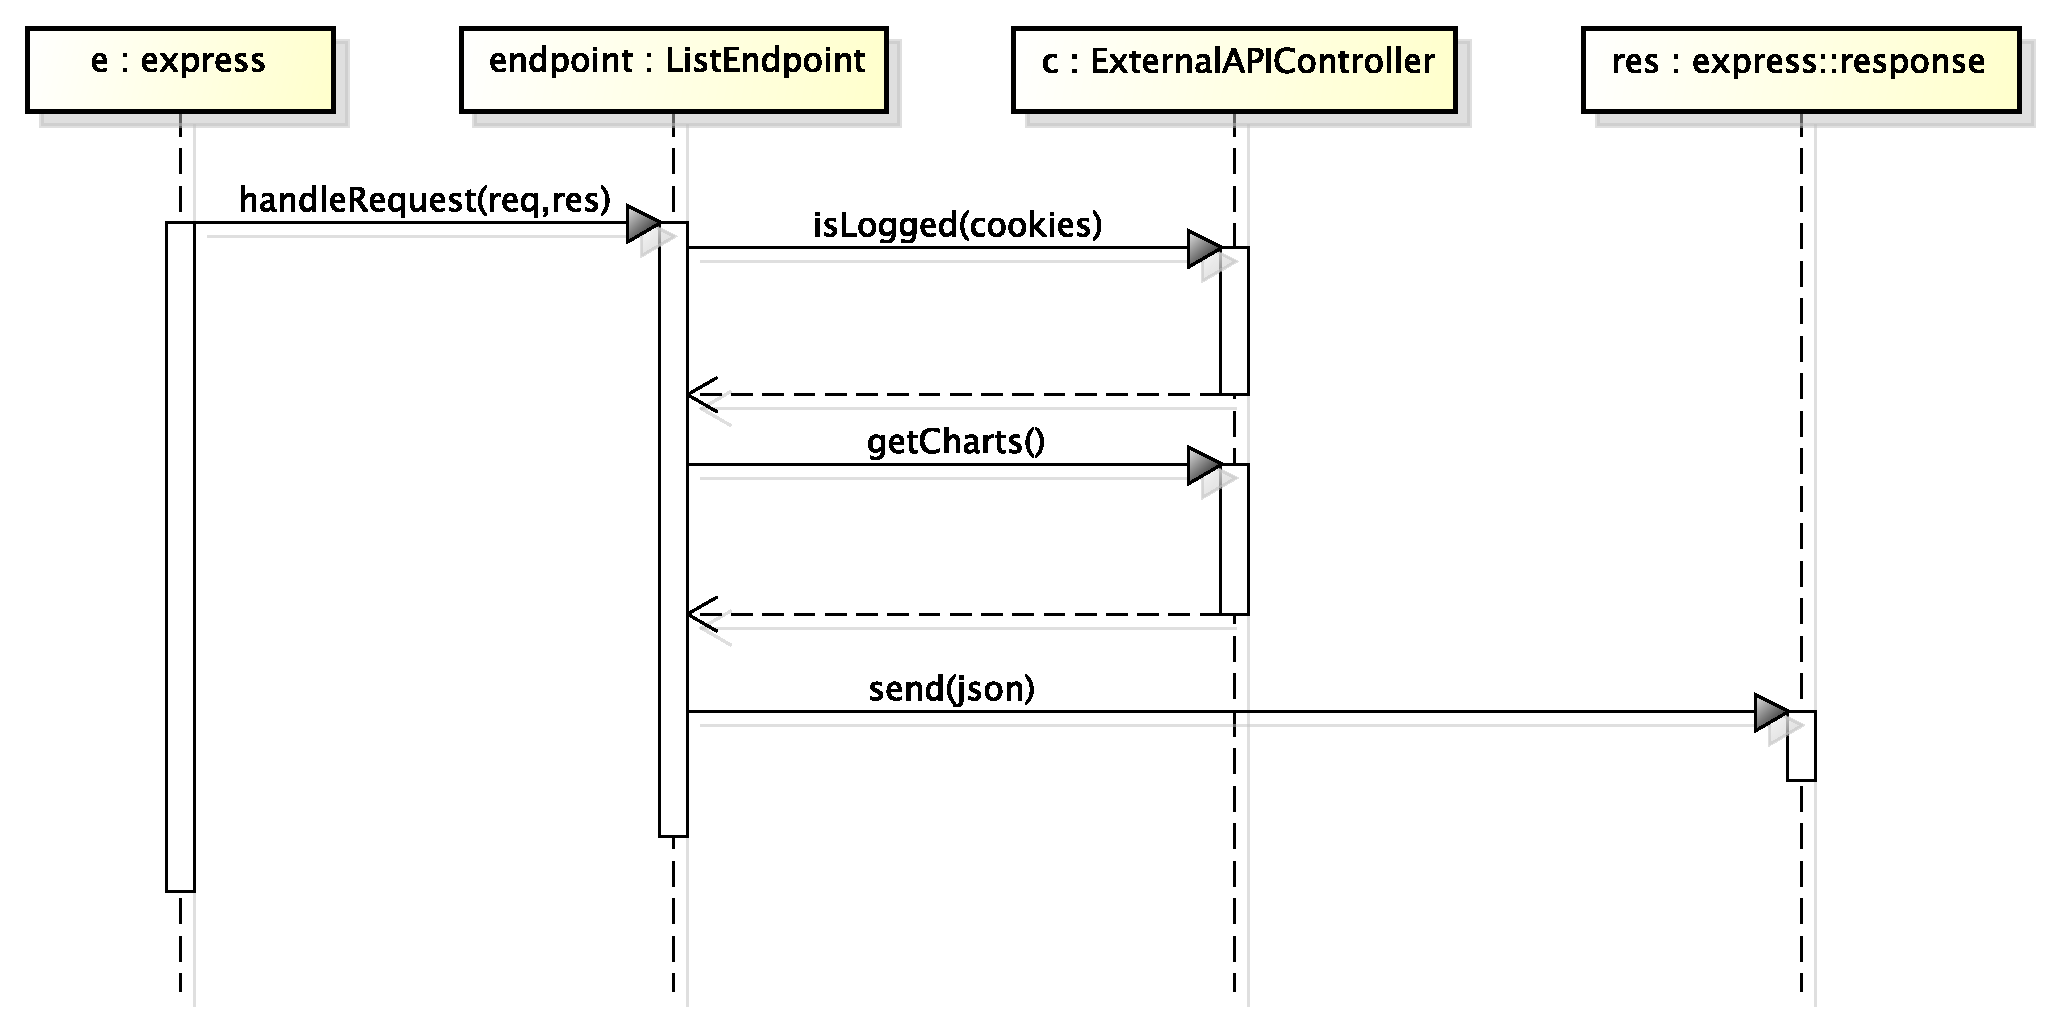
\includegraphics[scale=0.3]{DefinizioneDiProdotto/Pics/NorrisInvioLista}
                \caption{Diagramma di sequenza - Norris, invio lista}
            \end{figure}

            
        \level{3}{Invio di un chart}
        	Tale diagramma descrive come viene gestita la richiesta di un chart da parte di un \insglo{client} dal sistema \insglo{Norris}.
            \begin{figure}[H]
                \centering
                \includegraphics[scale=0.3]{DefinizioneDiProdotto/Pics/NorrisInvioChart}
                \caption{Diagramma di sequenza - Norris, invio chart}
            \end{figure}

	\level{2}{Chuck}
	\begin{figure}[H]\centering
        \includegraphics[width=\textwidth]{SpecificaTecnica/Pics/componentiChuck}
        \caption{Diagramma delle componenti di Chuck}
    \end{figure}
	\level{3}{Design Pattern utilizzati}
	Nella progettazione delle componenti di Chuck abbiamo deciso di utilizzare il design pattern MVC.
	MOTIVAZIONE
    \level{3}{Descrizione dei componenti di Chuck}
    	\level{4}{Chuck API Manager}
    		La componente Chuck Api Manager si occupa di implementare le funzionalità offerte dalle API di Chuck allo sviluppatore client. Queste funzionalità sono:
    		\begin{itemize}
						\item inserimento di nuovi grafici in un sito web;
						\item scelta del tag HTML in cui inserire un grafico;
						\item modifica di alcune impostazioni dei grafici;
						\item login;
						\item logout.
			\end{itemize}
    		Questa componente si occupa inoltre di gestire la comunicazione con Norris.
    		
    	\level{4}{Chart View}
    	La componente Chart View ha il compito di visualizzare i grafici all'interno della pagina web. I grafici possono essere del tipo Bar Chart, Line Chart, Map Chart e Table. Quando un grafico viene aggiornato, questa componente si occupa di aggiornare anche la sua visualizzazione nella pagina web.

    	\level{4}{Controller}
    	La componente Controller ha lo scopo di ricevere gli input provenienti dalla Chart View ed effettuarne la gestione. L'input consiste in un sottoinsieme di dataset scelti dall'utente che sta visualizzando la pagina web. Il Controller deve far sì che vengano visualizzati solo questi dataset, in modo da permettere all'utente di applicare un filtro sulle serie.

    	\level{4}{Data Model}
    	La componente Data Model è un modello che astrae i grafici visualizzati nella pagina web. In essa sono contenuti i dati riguardanti i grafici, assieme alle relative impostazioni. In particolare sono presenti i modelli di tutte le tipologie di chart implementati da Norris. Il Data Model fornisce per ciascuna tipologia di grafico i metodi per inserire i dati e configurare alcune impostazioni. 
    
	\level{3}{Descrizione delle interazioni tra le componenti}
	
		\level{4}{Chuck API Manager - Data Model}
		Quando il Web Developer utilizza le API di Chuck oppure quando arriva un messaggio da Norris, Chuck API Manager apporta le opportune modifiche al Data Model, in modo che quest'ultimo rispecchi costantemente lo stato dei grafici da visualizzare.

		\level{4}{Chart View - Data Model}
		Quando la Chart View deve aggiornare la visualizzazione del grafico, essa effettua una query sul Data Model per ottenere le nuove informazioni relative al grafico da aggiornare.

		\level{4}{Data Model - Chart View}
		Quando avviene una modifica nel Data Model, una notifica avvisa la Chart View dell'avvenuto cambiamento. In particolare ciò accade quando è stato inserito un nuovo grafico o quando è arrivato l'aggiornamento di un grafico già presente.

		\level{4}{Chart View - Controller}
		Quando la Chart View riceve un input dall'utente, una notifica avvisa il Controller in modo che intraprenda l'azione per gestirla.

		\level{4}{Controller - Chart View}
		In caso di necessità il controller può selezionare la Chart View da visualizzare.
		\level{4}{Controller - Data Model}
		Quando intraprende un'azione, il controller può effettuare delle modifiche nel Data Model. In particolare ciò accade quando si deve inserire un nuovo grafico o quando arriva l'aggiornamento di un grafico già presente.

	\level{2}{Applicazione Android}
	\begin{figure}[H]\centering
        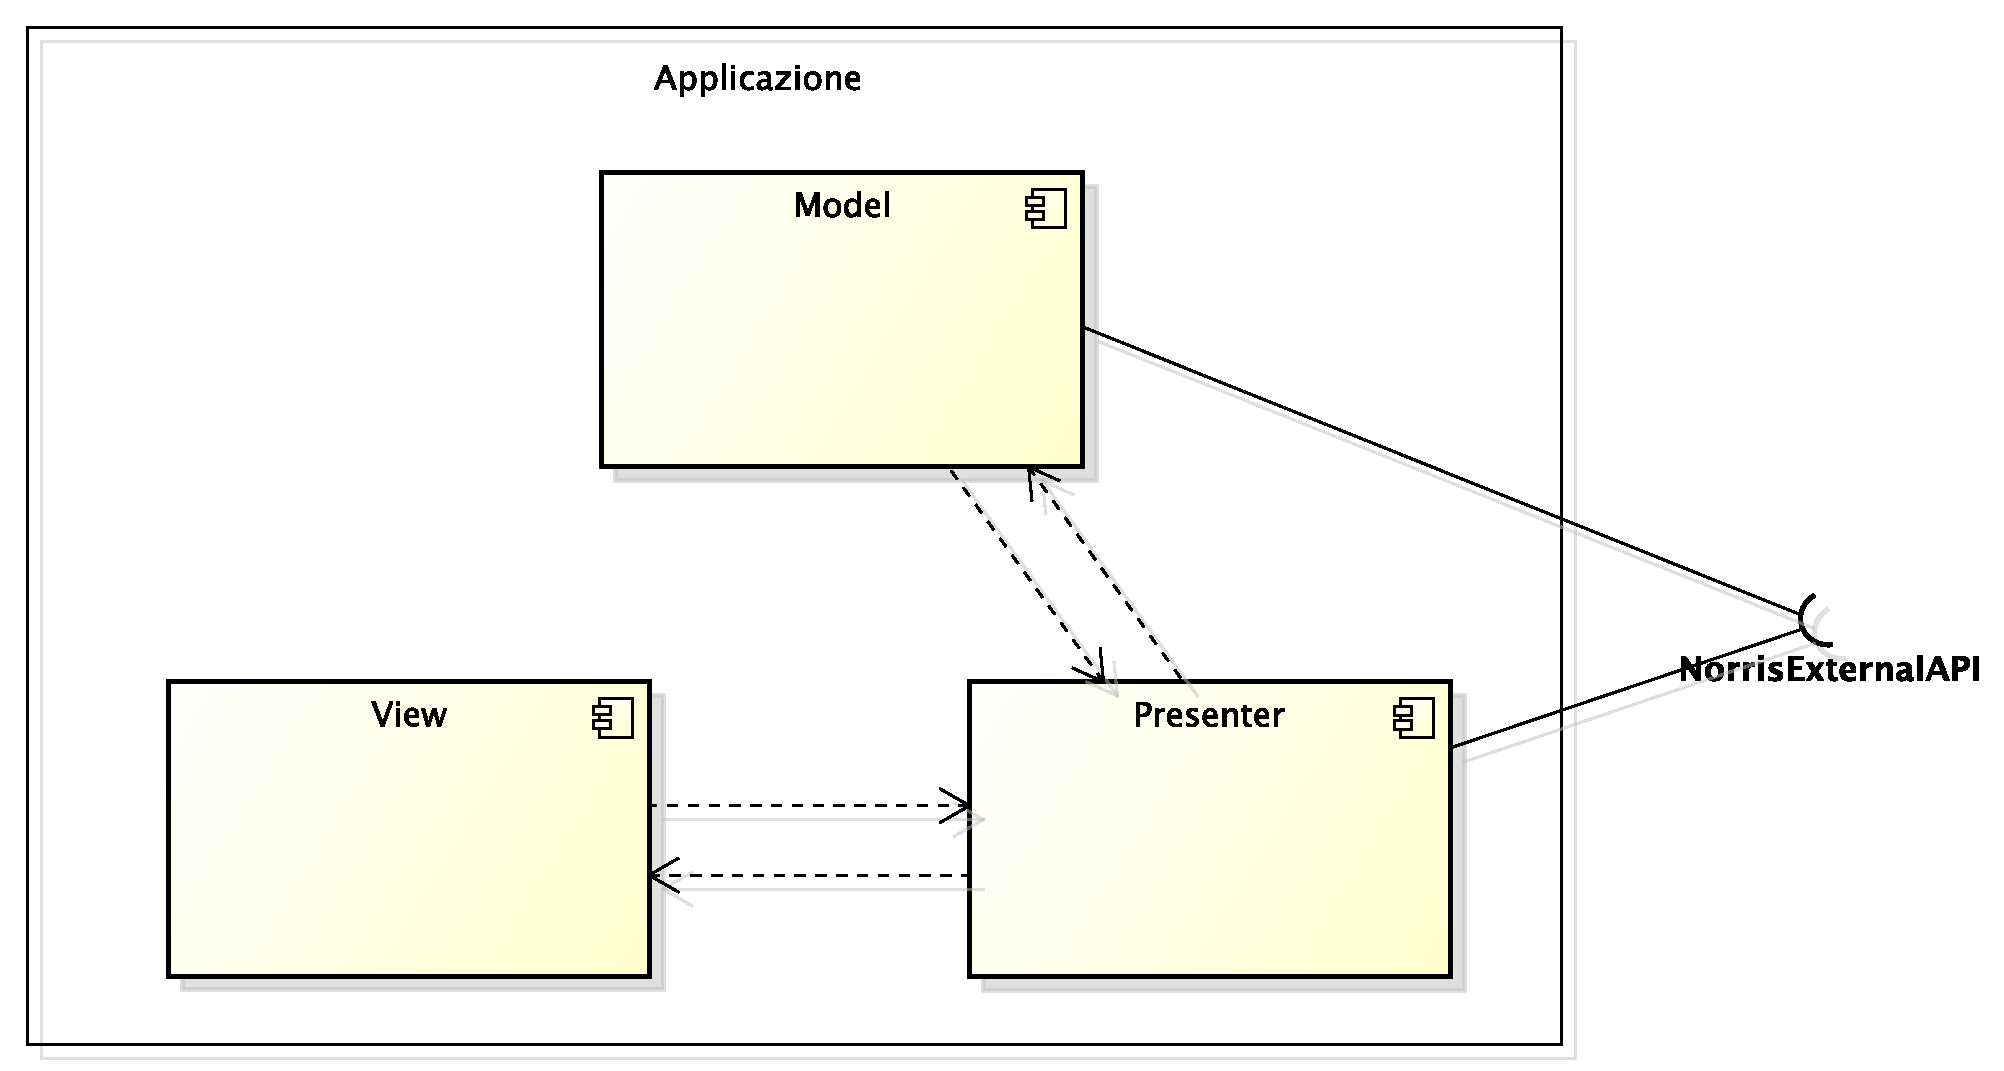
\includegraphics[width=\textwidth]{SpecificaTecnica/Pics/ComponentiApplicazione}
        \caption{Diagramma delle componenti dell'Applicazione Android}
    \end{figure}
    \level{3}{Descrizione delle componenti dell'Applicazione}
    	\level{4}{Model} 
        Il Model è la componente che rappresenta l'astrazione dei grafici visualizzati nell'applicazione. In essa sono contenuti i dati riguardanti i grafici, assieme alle relative impostazioni. In particolare sono presenti i modelli di tutte le tipologie di chart implementati da Norris. Il Data Model fornisce per ciascuna tipologia di grafico i metodi per inserire i dati e configurare alcune impostazioni. 
    
       \level{4}{View}
        La View è il componente che rappresenta le varie UI dell'applicazione e i vari widget dei grafici da inserire nelle UI. In tale componente potrebbero esser sollevati degli eventi scatenati dall'utente.
       \level{4}{Controller}
        Questo componente ha il compito di gestire tutto il controllo dell'applicazione. Le operazioni che esso gestisce sono riassunte nel seguente elenco:
        	\begin{itemize}
        		\item creazione del modello qualora questo sia necessario;
        		\item utilizzo delle API esterne di Norris;
        		\item interpretazione dei pacchetti ricevuti dal server contenenti i dati delle richieste API;
        		\item ascolto sul canale socket per ricevere gli aggiornamenti di stato dei chart;
        		\item interpretazione dei pacchetti di aggiornamento;
        		\item richiesta al modello di aggiornare il proprio stato;
        		\item richiesta della creazione dei widget dei grafici da inserire nelle UI dell'applicazione;
        		\item avvio delle varie activity dell'applicazione;
        		\item gestione delle gesture dell'utente.
        \end{itemize}
    \level{3}{Descrizione delle interazioni tra le componenti}
    	Le interazioni tra i componenti sono rappresentati con una freccia. Sono presenti due tipologie di frecce:
    	\begin{itemize}
    			\item{continua: } rappresenta l'invocazione di un metodo;
    			\item{tratteggiata: } rappresenta lo scatenarsi di un evento.
    		\end{itemize}

    	Riportiamo di seguito la descrizione di ogni interazione.

    	\level{4}{View - Controller}
        In seguito all'esecuzione di una gesture da parte dell'utente, la View notifica il Controller tramite l'emissione dell'evento opportuno. Il Controller si occupa quindi di gestire quest'ultimo. Questa interazione si verifica in particolare quando l'utente seleziona un item della lista dei grafici presenti nell'istanza di Norris richiesta.

	    \level{4}{Controller - Model}
	    Il Controller richiede al Model di modificare il proprio stato. Ciò avviene per esempio subito dopo l'utilizzo dell'API esterna di Norris per richiedere un grafico o in seguito all'arrivo di un pacchetto di aggiornamento.

	    \level{4}{Model - View}
	    Il Model notifica le View che lo osservano ogniqualvolta il suo stato viene modificato. Tale interazione è neccessaria per mantenere coerenza tra il modello e la sua rappresentazione nella View. 

	    \level{4}{View - Model}
	   	Questa interazione rappresenta la richiesta dello stato del Model da parte della View. Viene effettuata quando la View ha la necessità di esporre i dati del Model o qualcosa che sia dipendente dallo stato di quest'ultimo. Ciò si verifica per esempio subito dopo che la View ha ricevuto la notifica di aggiornamento da parte del modello.

	    \level{4}{Controller - View}
	   	Tale interazione rappresenta la richiesta da parte del Controller di visualizzare una specifica Activity. Ciò avviene ad ogni necessità di cambiare Activity.
        
    \level{3}{Design pattern utilizzati}
    Nella progettazione delle componenti dell'applicazione Android abbiamo deciso di utilizzare i seguenti pattern architetturali:
        \level{4}{Model View Controller}
        Model-View-Controller (MVC) è un pattern architetturale utilizzato per separare il codice in blocchi di funzionalità ben distinte.\\
        Per la descrizione del pattern e dei vantaggi derivanti dalla sua applicazione si rimanda all'appendice \nameref{app:MVC}.
        \level{5}{Contesto di utilizzo}
        L'MVC viene utilizzato per dividere le classi dell'applicazione Android in tre grandi componenti:
        \begin{itemize}
        \item Model;
        \item View;
        \item Controller;
        \end{itemize}


	\level{2}{Dashboard APS}
	La \insglo{dashboard} è un esempio d'uso di \insglo{Norris}: rappresenta un modo in cui il \insglo{prodotto} può essere utilizzato. Essa, dunque, è una pagina web generata in automatico dal \insglo{server} \insglo{Norris}. Essa è costituita da più grafici che l'utente finale potrà visualizzare sul proprio \insglo{browser}. Di seguito viene fornito un \insglo{mockup} della pagina, che mostra a grandi linee come sarà visualizzata la \insglo{dashboard} una volta completata..
	\begin{figure}[H]\centering
        \includegraphics[width=\textwidth]{SpecificaTecnica/Pics/DashboardMockup}
        \caption{Mockup della dashboard APS}
    \end{figure}
    Vengono ora descritti i vari componenti di cui è fatta la pagina, ovvero vengono descritti i grafici che sono stati inseriti all'interno del \insglo{mockup} mostrato in precedenza.
    \level{3}{Descrizione delle componenti della Dashboard}
    	\level{4}{Map chart}
    		Tramite questo grafico l'utilizzatore della \insglo{dashboard} è in grado di visualizzare in tempo reale la posizione di tutti i bus attivi nelle varie linee dell'\insglo{APS}. Tale grafico mette inoltre a disposizione dell'utente delle opzioni riguardanti il filtraggio delle linee presenti: infatti, esso permette di scegliere le linee che si intendono visualizzare, semplicemente nascondendo e ignorando le rimanenti. In questo modo si può trasformare un grafico potenzialmente caotico (a causa della grande quantità di punti presenti al suo interno) in un molto più comprensibile e consultabile.
    	\level{4}{Table}
    		Tale grafico è dedicato ai punti di maggior interesse di Padova. Esso fornisce all'utente utilizzatore della \insglo{dashboard} il tempo necessario all'arrivo degli autobus in alcune fermate \insglo{APS} molto frequentate. In particolare, è possibile visualizzare quanto tempo manca all'arrivo del prossimo autobus in una determinata stazione, e a quale linea il suddetto autobus appartiene. Grazie ad esso gli utenti sono in grado di capire quanto devono attendere mediamente prima di poter salire su uno dei mezzi da loro scelti.
    	\level{4}{Bar chart}
    		Questo grafico permette all'utilizzatore della \insglo{dashboard} di visualizzare quanti autobus sono attivi su ciascuna linea dell'\insglo{APS}. Tale grafico mette inoltre a disposizione dell'utente delle opzioni riguardanti il filtraggio delle linee presenti: infatti, esso permette di scegliere le linee di cui si vuole visualizzare il numero di bus attivi. Grazie a questo grafico, l'utente può ottenere utili informazioni su quanto una linea è frequentata e sul tempo di attesa che mediamente passa tra làarrivo di un mezzo e del successivo.
    \level{3}{Creazione della Dashboard}
        In questa sezione viene mostrato quali sono i passi principali che l'utilizzatore di \insglo{Norris} deve fare per creare la \insglo{Dashboard} \insglo{APS}. La descrizione che segue può essere maggiormente compresa grazie al diagramma delle attività qui presente.
        \begin{figure}[H]\centering
            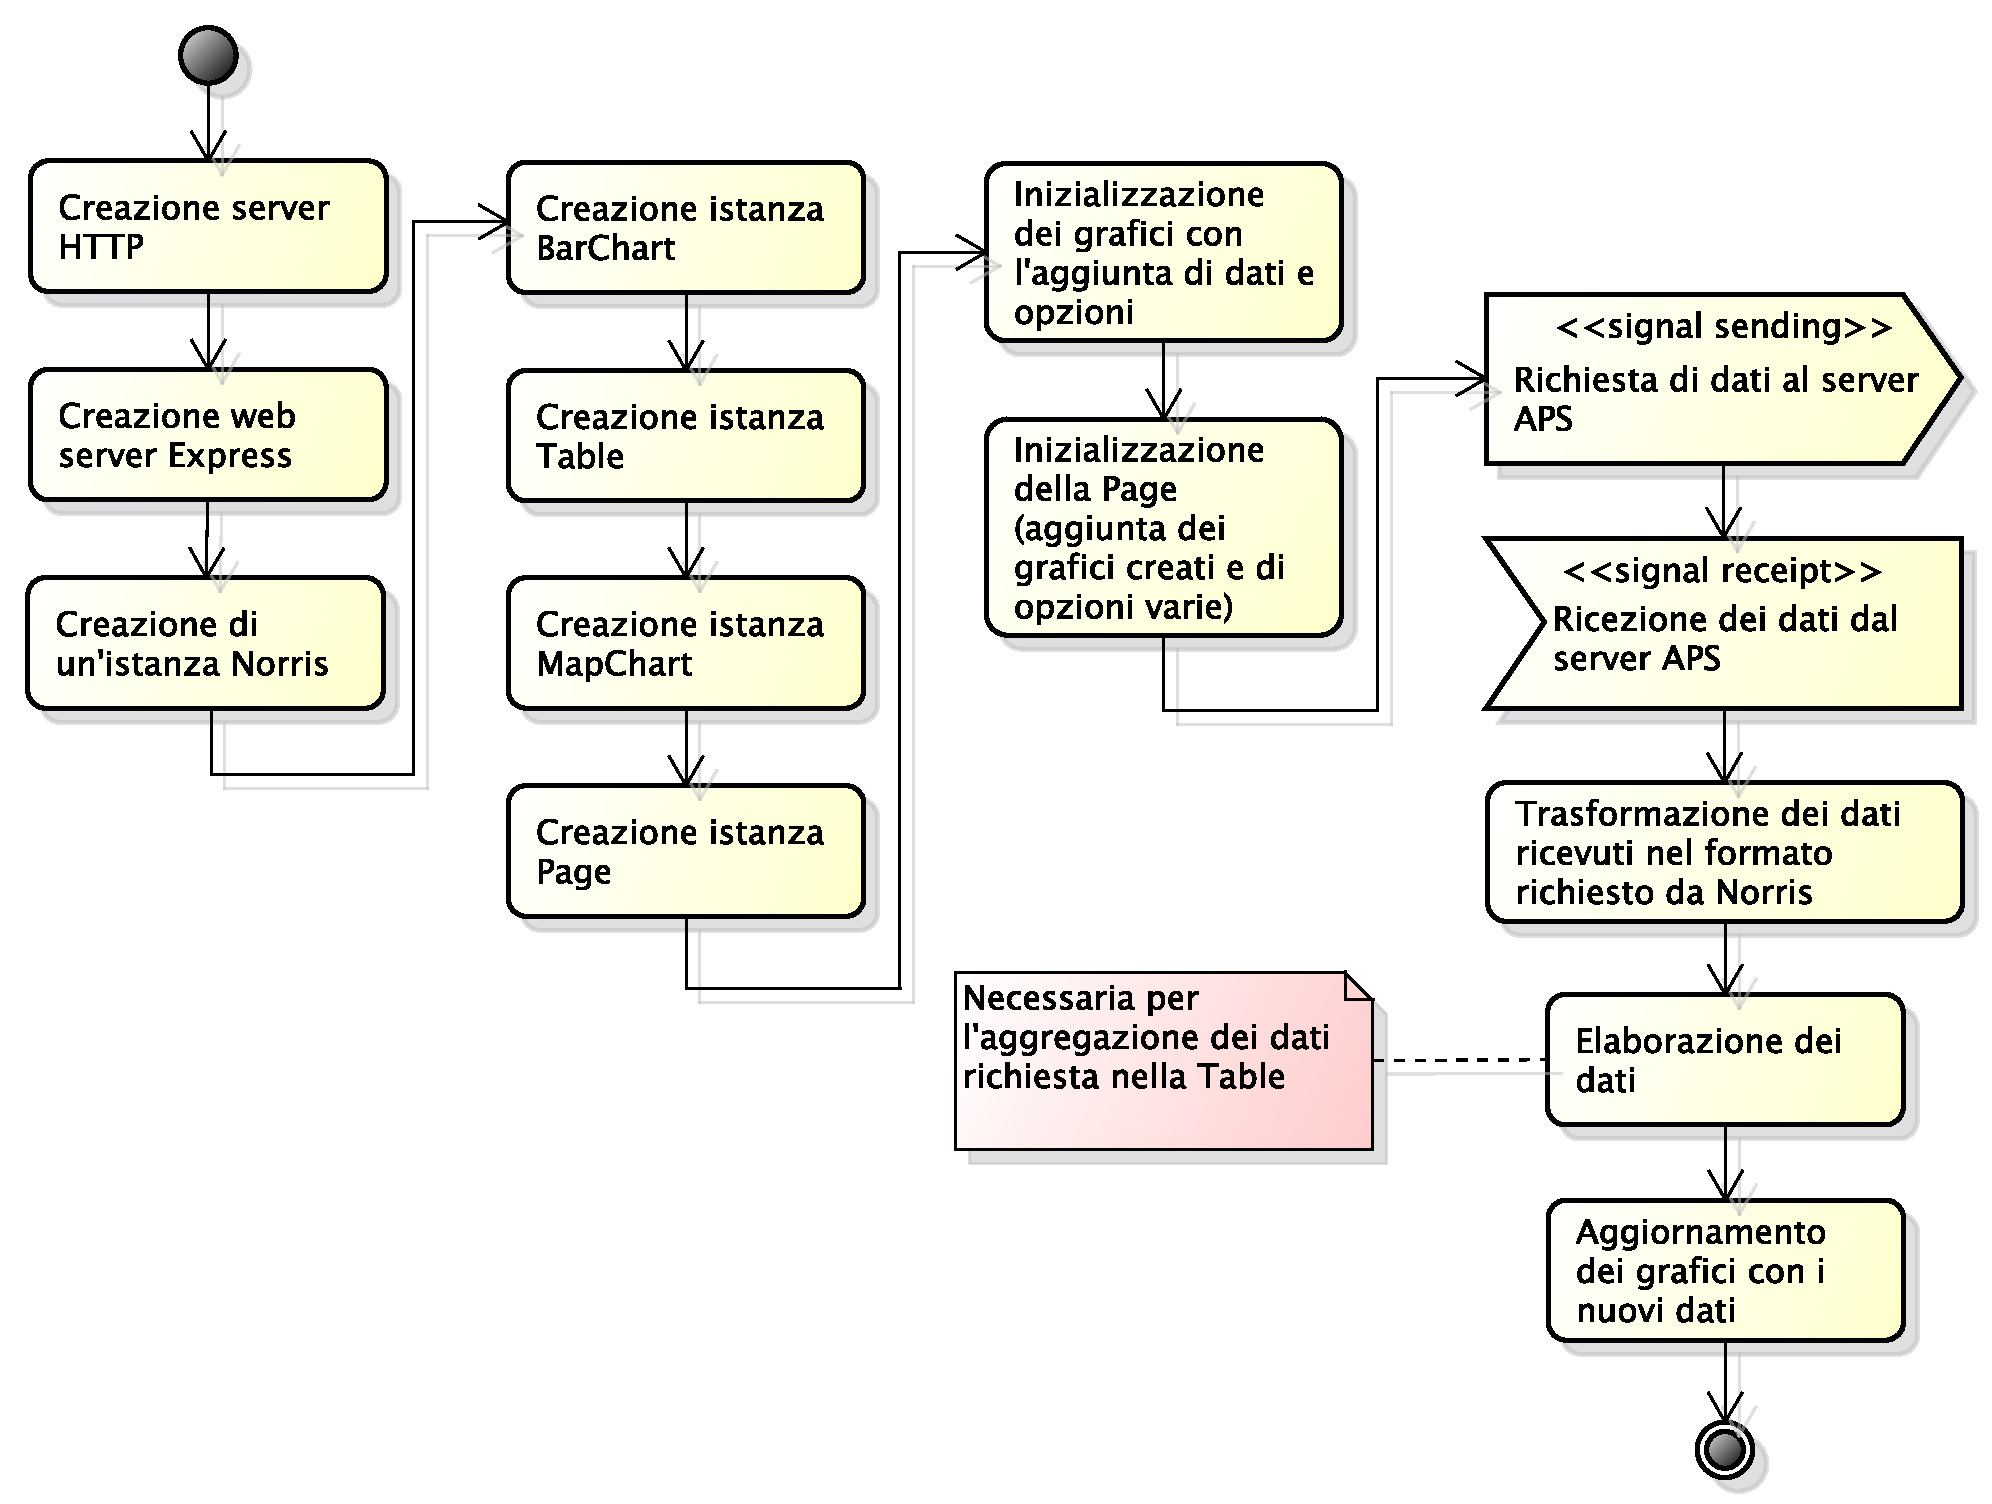
\includegraphics[width=\textwidth]{SpecificaTecnica/Pics/CreateDashboard}
            \caption{Creazione della Dashboard - diagramma delle attività}
        \end{figure}
        \begin{enumerate}
            \item Requisito fondamentale per la creazione della \insglo{dashboard} è che esista e sia correttamente funzionante un'istanza di \insglo{Norris}. Dunque, seppur banale, la prima cosa che l'utilizzatore di \insglo{Norris} deve fare è assicurarsi di ciò.
            \item In secondo luogo vanno creati i grafici che dovranno essere contenuti nella pagina web. Essi inizialmente sono vuoti (sono privi di impostazioni e di dati, che verranno aggiunti successivamente). Lo sviluppatore fa uso dell'interfaccia \texttt{\insglo{Norris}::InternalAPIManager::\insglo{Norris}} per fare ciò. Essa è presentata e descritta all'interno di questo documento (vedi progettazione architetturale di \insglo{Norris}).
            \item A questo punto va creata la pagina che dovrà contenere i grafici creati in precedenza. Inizialmente, dunque, anch'essa sarà vuota, ovvero priva di contenuto (i grafici) e di opzioni. Per creare la pagina va utilizzata ancora una volta l'interfaccia disponibile allo sviluppatore \texttt{\insglo{Norris}::InternalAPIManager::\insglo{Norris}} (vedi progettazione architetturale di \insglo{Norris}).
            \item Compito dello sviluppatore è ora quello di inizializzare i grafici creati in precedenza, mediante l'aggiunta di eventuali dati e impostazioni.
            \begin{itemize}
                \item Per quanto riguarda il BarChart e il MapChart essi saranno inizialmente vuoti. Infatti, i dati verranno aggiunti mano a mano che verranno ricevuti dai \insglo{server} dell'\insglo{APS}, in un momento successivo.\\
                Le impostazioni, invece, possono già essere scelte per entrambi i chart (per esempio il titolo, la descrizione, la posizione della legenda ecc.).\\
                Sia per inserire un insieme vuoto di dati iniziali, sia per impostare le opzioni dei grafici, si fa uso dell'interfaccia \texttt{\insglo{Norris}::InternalAPIManager::Chart}, descritta e documentata all'interno del presente documento (vedi progettazione architetturale \insglo{Norris}).
                \item La \insglo{Table}, invece, inizialmente non sarà del tutto vuota (seppur inutilizzabile). Infatti, nonostante non si conoscano ancora le posizioni dei vari mezzi dell'\insglo{APS}, si devono inserire i nomi dei punti di interesse che si vogliono monitorare successivamente. Ci si deve contemporaneamente preoccupare di rendere evidente il fatto che non siano ancora disponibili dati su cui basare i calcoli del tempo medio di attesa (per esempio impostando il valore “unknown” nei campi “Linea del prossimo bus in arrivo” e “tempo di attesa medio”).\\
                Per quanto riguarda le impostazioni, esse possono essere scelte liberamente dallo svilupparoe.\\
                Sia per inserire i dati iniziali, sia per impostare le opzioni del grafico, si fa uso dell'interfaccia \texttt{\insglo{Norris}::InternalAPIManager::Chart}, descritta e documentata all'interno del presente documento (vedi progettazione architetturale \insglo{Norris}).
            \end{itemize}
            \item Dopo aver inizializzato i grafici in modo corretto, lo sviluppatore li inserisce all'interno della pagina creata in precedenza. Egli può inoltre scegliere liberamente le impostazioni della pagina.\\
            Lo sviluppatore fa uso dell'interfaccia \texttt{\insglo{Norris}::InternalAPIManager::Page} per eseguire questi compiti. Tale interfaccia è presentata e descritta all'interno di questo documento (vedi progettazione architetturale di \insglo{Norris}).
            \item Ora che tutti i vari elementi sono stati correttamente inizializzati, allo sviluppatore non resta che tenere costantemente aggiornati i dati contenuti all'interno dei grafici (e dunque della pagina). Per fare ciò, egli deve innanzitutto preoccuparsi di richiedere i dati riguardanti le varie linee al \insglo{server} dell'\insglo{APS}.
            \item Una volta ottenuti i dati, lo sviluppatore si deve preoccupare di convertirli in un formato fruibile da \insglo{Norris}. Essi, infatti, sono nel formato fornito dall'\insglo{APS}, che non necessariamente è lo stesso di quello utilizzato dai nostri prodotti.
            \item I dati a questo punto vanno aggregati e/o elaborati nel modo richiesto dai vari grafici presenti.
            \begin{itemize}
                \item Per la \insglo{Table} si devono utilizzare i dati a disposizione per capire il mezzo più vicino a un dato punto e per calcolare il tempo medio di attesa.
                \item Per il \insglo{Bar Chart} si devono utilizzare i dati a disposizione per calcolare quanti mezzi sono attivi al momento per ciascuna linea presente.
            \end{itemize}
            \item Infine, grazie ai dati ottenuti e ai calcoli eseguiti precedentemente, lo sviluppatore è in grado di aggiornare i vari grafici. Gli aggiornamenti avvengono in base alla tipologia di grafico e in base ai risultati che sono stati ottenuti precedentemente.\\
            Prima di cominciare un nuovo processo di aggiornamento (tramite la richiesta di dati al \insglo{server} \insglo{APS}), si attende per un tempo prefissato (minore è il tempo di aggiornamento, maggiore sarà la reattività e la precisione della \insglo{Dashboard}).
        \end{enumerate}
	
		\newpage
		\level{1}{Stime di fattibilità e di bisogno di risorse}
Dopo aver definito l'architettura a un sufficiente livello di dettaglio, il team di sviluppo è in grado di fornire una stima della fattibilità.\\
Grazie alle tecnologie individuate si prevede di riuscire ad adempiere a tutte le richieste fatte dal proponente.\\
In questi mesi, infatti, il gruppo ha studiato le tecnologie necessarie per implementare il prodotto, prima sconosciute, capendo il loro utilizzo e i loro pregi e difetti, grazie anche all'interazione col proponente. Anche il fatto che uno dei membri del team stia seguendo un corso di Programmazione Embedded ha aiutato molto nella realizzazione dell'architettura dell'applicazione Android richiesta. \\
Altri fattori che ci avvantaggiano sono che l'architettura del prodotto richiesto sia simile a quella di altri prodotti sul mercato, come Agenda (\url{https://github.com/rschmukler/agenda}), e la presenza in rete di numerose librerie per la gestione della parte grafica ed esempi sull'implementazione degli aggiornamenti in tempo reale.\\
Nell'ottica della suddivisione del lavoro, il fatto che il prodotto abbia un elevato livello di modularità agevolerà il \insrole{Responsabile di Progetto} nell'assegnazione dei prossimi task di codifica.\\
	
		\newpage
		\level{1}{Tracciamento}
	\level{2}{Componenti-Requisiti}
	
				\begin{longtabu} spread 1cm [c]{|X[l]|X[l]|X[l]|}
					\hline
					\rowfont{\bf \centering}
					Codice &
					Dettaglio &
					Requisiti abbinati \\
					\hline
					\endhead
					
					N001 & Norris::InternalAPIManager & \parbox[t]{4cm}{ RRF1 \\ RRF1.1 \\ RRF1.2 \\ RRF1.3 \\ RRF1.4 \\ RRF1.5 \\ RRF1.5.1 \\ RRF1.5.1.1 \\ RRF1.5.1.2 \\ RRF1.5.2 \\ RRF1.5.2.2 \\ RRF1.5.3 \\ RRF1.5.3.1 \\ RRF1.5.3.2 \\ RDF1.5.4 \\ RRF1.5.5 \\ RRF1.5.5.1 \\ RRF1.5.5.2 \\ RRF1.5.6 \\ RRF1.5.6.1 \\ RRF1.5.6.2 \\ RRF1.5.7 \\ RRF1.5.7.1 \\ RRF1.5.7.2 \\ RDF1.5.7.3 \\ RRF1.5.7.4 \\ RDF1.5.7.5 \\ RDF1.5.7.6 \\ RRF1.5.7.7 \\ RRF1.5.8 \\ RRF1.5.9 \\ RRF1.5.10 \\ RRF1.5.11 \\ RRF1.5.12 \\ RRF1.5.13 \\ RRF1.5.14 \\ RRF1.5.15 \\ RRF1.5.16 \\ RRF1.5.17 \\ RRF1.5.18 \\ RRF1.5.18 \\ RRF1.5.19 \\ RRF1.5.20 \\ RRF1.5.21 \\ RRF1.5.22 \\ RRF1.5.23 \\ RRF1.6 \\ RRF1.7 \\ RRF1.8} \\ \hline
                                        N001 & Norris::InternalAPIManager & \parbox[t]{4cm}{ RRF1.9 \\ RRF1.10 \\ RRF2 \\ RRF2.1 \\ RRF2.2 \\ RRF2.3 \\ RRF2.4 \\ RRF2.5 \\ RRF2.6 \\ RRF3 \\ RRF2.7 \\ RRF3.1 \\ RRF3.2 \\ RRF3.2.1 \\ RRF3.2.2 \\ RRF3.3 \\ RRF4 \\ RRC10 \\ RRF1.5.2.1 }\\
                \hline
                N002 & Norris::ExternalAPIManager & \parbox[t]{4cm}{ RRF5 \\ RRF5.1 \\ RRF5.1.1 \\ RRF5.3 \\ RRF5.4 \\ RRC10 \\ RRC11 \\ RRF9 \\ RRF6.4 \\ RRF6.3 \\ RRF8.3 }\\
                \hline
                N003 & Norris::DataModel & \parbox[t]{4cm}{ RRF1.4 \\ RRF1 \\ RRF1.1 \\ RRF1.2 \\ RRF1.3 \\ RRF1.5 \\ RRF1.5.1 \\ RRF1.5.1.1 \\ RRF1.5.1.2 \\ RRF1.5.2 \\ RRF1.5.2.2 \\ RRF1.5.3 \\ RRF1.5.3.1 \\ RRF1.5.3.2 \\ RDF1.5.4 \\ RRF1.5.5 \\ RRF1.5.5.1 \\ RRF1.5.5.2 \\ RRF1.5.6 \\ RRF1.5.6.1 \\ RRF1.5.6.2} \\ \hline 
                N003 & Norris::DataModel & \parbox[t]{4cm}{ RRF1.5.7 \\ RRF1.5.7.1 \\ RRF1.5.7.2 \\ RDF1.5.7.3 \\ RRF1.5.7.4 \\ RDF1.5.7.5 \\ RDF1.5.7.6 \\ RRF1.5.7.7 \\ RRF1.5.8 \\ RRF1.5.9 \\ RRF1.5.10 \\ RRF1.5.11 \\ RRF1.5.12 \\ RRF1.5.13 \\ RRF1.5.14 \\ RRF1.5.15 \\ RRF1.5.16 \\ RRF1.5.17 \\ RRF1.5.18 \\ RRF1.5.19 \\ RRF1.5.20 \\ RRF1.5.21 \\ RRF1.5.22 \\ RRF1.5.23 \\ RRF1.6 \\ RRF1.7 \\ RRF1.9 \\ RRF1.8 \\ RRF1.10 \\ RRF2 \\ RRF2.1 \\ RRF2.2 \\ RRF2.3 \\ RRF2.4 \\ RRF2.5 \\ RRF2.6 \\ RRF3 \\ RRF2.7 \\ RRF3.1 \\ RRF3.2 \\ RRF3.2.1 \\ RRF3.2.2 \\ RRF3.3 \\ RRF5 \\ RRF5.1 \\ RRF5.1.1 \\ RRF5.2 \\ RRF1.5.2.1 \\ RRF6.4 }\\
                \hline
                C001 & Chuck::Directive & \parbox[t]{4cm}{ RRF6 \\ RRF6.1 \\ RDF6.2.1 \\ RDF6.2.2 \\ RDF6.2.3 \\ RDF6.2.4 \\ RDF6.2.5 \\ RDF6.2.6 \\ RDF6.2.7 \\ RDF6.2.8 \\ RDF6.2.9 \\ RDF6.2.10 \\ RDF6.2.11 \\ RDF6.2.12 \\ RDF6.2.13 }\\
                \hline
                C002 & Chuck::View & \parbox[t]{4cm}{ RRF6 \\ RDC18 }\\
                \hline
                C003 & Chuck::ViewModel & \parbox[t]{4cm}{ RRF6 \\ RDF6.2.1 \\ RDF6.2.2 \\ RDF6.2.3 \\ RDF6.2.4 \\ RDF6.2.5 \\ RDF6.2.6 \\ RDF6.2.7 \\ RDF6.2.8 \\ RDF6.2.9 \\ RDF6.2.10 \\ RDF6.2.11 \\ RDF6.2.12 \\ RDF6.2.13 }\\
                \hline
                C004 & Chuck::Model & \parbox[t]{4cm}{ RRF6 \\ RDF6.2.1 \\ RDF6.2.2 \\ RDF6.2.3 \\ RDF6.2.4 \\ RDF6.2.5 \\ RDF6.2.6 \\ RDF6.2.7 \\ RDF6.2.8 \\ RDF6.2.9 \\ RDF6.2.10 \\ RDF6.2.11 \\ RDF6.2.12 \\ RDF6.2.13 \\ RDF6.2 \\ RRF6.4 }\\
                \hline
                A001 & Applicazione::Model & \parbox[t]{4cm}{ ROF8 \\ RRF8.2 \\ RRF8.4 \\ RRF8.5 }\\
                \hline
                A002 & Applicazione::View & \parbox[t]{4cm}{ ROF8 \\ RRF8.1 \\ RRF8.2 \\ RRF8.4 \\ RRF8.5 }\\
                \hline
                A003 & Applicazione::Presenter & \parbox[t]{4cm}{ ROF8 \\ RRF8.1 \\ RRF8.2 \\ RRF8.4 \\ RRF8.5 }\\
                \hline
                A004 & Applicazione::Model::NorrisChart & \parbox[t]{4cm}{ ROF8 }\\
                \hline
                A005 & Applicazione::Model::Service & \parbox[t]{4cm}{ ROF8 \\ RRF8.3 }\\
                \hline
                N004 & Norris::DataModel::NorrisChart & \parbox[t]{4cm}{ RRF1.6 }\\
                \hline
                N005 & Norris::DataModel::NorrisPage & \parbox[t]{4cm}{ RRF3 }\\
                \hline
                C005 & Chuck::Model::NorrisChart & \parbox[t]{4cm}{ RRF1 \\ RRF1.1 \\ RRF1.2 \\ RRF1.3 \\ RRF1.4 \\ RRF2 \\ RRF2.1 \\ RRF2.2 \\ RRF2.3 \\ RRF2.4 \\ RRF2.5 \\ RRF2.6 \\ RRF2.7 }\\
                \hline
                C006 & Chuck::Model::Services & \parbox[t]{4cm}{ RRF6.3 \\ RRC17 }\\
                \hline
                                \caption{Tracciamento componenti-requisiti}
				\end{longtabu}
				
	\level{2}{Requisiti-Componenti}
	
				\begin{longtabu} spread 1cm [c]{|X[l]|X[l]|}
					\hline
					\rowfont{\bf \centering}
					Requisito &
					Componente \\
					\hline
					\endhead
					
					RRF1 & \parbox[t]{4cm}{ N001 \\ N003 \\ C005 } \\ 
                \hline
                RRF1.1 & \parbox[t]{4cm}{ N001 \\ N003 \\ C005 } \\ 
                \hline
                RRF1.5 & \parbox[t]{4cm}{ N001 \\ N003 } \\ 
                \hline
                RRF1.5.17 & \parbox[t]{4cm}{ N001 \\ N003 } \\ 
                \hline
                RRF1.5.1 & \parbox[t]{4cm}{ N001 \\ N003 } \\ 
                \hline
                RRF1.5.1.1 & \parbox[t]{4cm}{ N001 \\ N003 } \\ 
                \hline
                RRF1.5.1.2 & \parbox[t]{4cm}{ N001 \\ N003 } \\ 
                \hline
                RRF1.5.5 & \parbox[t]{4cm}{ N001 \\ N003 } \\ 
                \hline
                RRF1.5.5.1 & \parbox[t]{4cm}{ N001 \\ N003 } \\ 
                \hline
                RRF1.5.5.2 & \parbox[t]{4cm}{ N001 \\ N003 } \\ 
                \hline
                RDF1.5.4 & \parbox[t]{4cm}{ N001 \\ N003 } \\ 
                \hline
                RRF1.5.18 & \parbox[t]{4cm}{ N001 \\ N001 \\ N003 } \\ 
                \hline
                RRF1.5.7 & \parbox[t]{4cm}{ N001 \\ N003 } \\ 
                \hline
                RRF1.5.7.1 & \parbox[t]{4cm}{ N001 \\ N003 } \\ 
                \hline
                RRF1.5.7.2 & \parbox[t]{4cm}{ N001 \\ N003 } \\ 
                \hline
                RDF1.5.7.3 & \parbox[t]{4cm}{ N001 \\ N003 } \\ 
                \hline
                RRF1.5.7.4 & \parbox[t]{4cm}{ N001 \\ N003 } \\ 
                \hline
                RDF1.5.7.6 & \parbox[t]{4cm}{ N001 \\ N003 } \\ 
                \hline
                RRF1.5.7.7 & \parbox[t]{4cm}{ N001 \\ N003 } \\ 
                \hline
                RDF1.5.7.5 & \parbox[t]{4cm}{ N001 \\ N003 } \\ 
                \hline
                RRF1.5.8 & \parbox[t]{4cm}{ N001 \\ N003 } \\ 
                \hline
                RRF1.5.21 & \parbox[t]{4cm}{ N001 \\ N003 } \\ 
                \hline
                RRF1.5.9 & \parbox[t]{4cm}{ N001 \\ N003 } \\ 
                \hline
                RRF1.5.10 & \parbox[t]{4cm}{ N001 \\ N003 } \\ 
                \hline
                RRF1.5.11 & \parbox[t]{4cm}{ N001 \\ N003 } \\ 
                \hline
                RRF1.5.12 & \parbox[t]{4cm}{ N001 \\ N003 } \\ 
                \hline
                RRF1.5.13 & \parbox[t]{4cm}{ N001 \\ N003 } \\ 
                \hline
                RRF1.5.14 & \parbox[t]{4cm}{ N001 \\ N003 } \\ 
                \hline
                RRF1.5.15 & \parbox[t]{4cm}{ N001 \\ N003 } \\ 
                \hline
                RRF1.5.16 & \parbox[t]{4cm}{ N001 \\ N003 } \\ 
                \hline
                RRF1.5.2 & \parbox[t]{4cm}{ N001 \\ N003 } \\ 
                \hline
                RRF1.5.2.1 & \parbox[t]{4cm}{ N001 \\ N003 } \\ 
                \hline
                RRF1.5.2.2 & \parbox[t]{4cm}{ N001 \\ N003 } \\ 
                \hline
                RRF1.5.3 & \parbox[t]{4cm}{ N001 \\ N003 } \\ 
                \hline
                RRF1.5.3.1 & \parbox[t]{4cm}{ N001 \\ N003 } \\ 
                \hline
                RRF1.5.3.2 & \parbox[t]{4cm}{ N001 \\ N003 } \\ 
                \hline
                RRF1.5.6 & \parbox[t]{4cm}{ N001 \\ N003 } \\ 
                \hline
                RRF1.5.6.1 & \parbox[t]{4cm}{ N001 \\ N003 } \\ 
                \hline
                RRF1.5.6.2 & \parbox[t]{4cm}{ N001 \\ N003 } \\ 
                \hline
                RRF1.5.19 & \parbox[t]{4cm}{ N001 \\ N003 } \\ 
                \hline
                RRF1.5.20 & \parbox[t]{4cm}{ N001 \\ N003 } \\ 
                \hline
                RRF1.5.22 & \parbox[t]{4cm}{ N001 \\ N003 } \\ 
                \hline
                RRF1.5.23 & \parbox[t]{4cm}{ N001 \\ N003 } \\ 
                \hline
                RRF1.6 & \parbox[t]{4cm}{ N001 \\ N003 \\ N004 } \\ 
                \hline
                RRF1.2 & \parbox[t]{4cm}{ N001 \\ N003 \\ C005 } \\ 
                \hline
                RRF1.3 & \parbox[t]{4cm}{ N001 \\ N003 \\ C005 } \\ 
                \hline
                RRF1.4 & \parbox[t]{4cm}{ N001 \\ N003 \\ C005 } \\ 
                \hline
                RRF1.7 & \parbox[t]{4cm}{ N001 \\ N003 } \\ 
                \hline
                RRF1.8 & \parbox[t]{4cm}{ N001 \\ N003 } \\ 
                \hline
                RRF1.9 & \parbox[t]{4cm}{ N001 \\ N003 } \\ 
                \hline
                RRF1.10 & \parbox[t]{4cm}{ N001 \\ N003 } \\ 
                \hline
                RRF2 & \parbox[t]{4cm}{ N001 \\ N003 \\ C005 } \\ 
                \hline
                RRF2.1 & \parbox[t]{4cm}{ N001 \\ N003 \\ C005 } \\ 
                \hline
                RRF2.2 & \parbox[t]{4cm}{ N001 \\ N003 \\ C005 } \\ 
                \hline
                RRF2.3 & \parbox[t]{4cm}{ N001 \\ N003 \\ C005 } \\ 
                \hline
                RRF2.4 & \parbox[t]{4cm}{ N001 \\ N003 \\ C005 } \\ 
                \hline
                RRF2.5 & \parbox[t]{4cm}{ N001 \\ N003 \\ C005 } \\ 
                \hline
                RRF2.6 & \parbox[t]{4cm}{ N001 \\ N003 \\ C005 } \\ 
                \hline
                RRF2.7 & \parbox[t]{4cm}{ N001 \\ N003 \\ C005 } \\ 
                \hline
                RRF3 & \parbox[t]{4cm}{ N001 \\ N003 \\ N005 } \\ 
                \hline
                RRF3.1 & \parbox[t]{4cm}{ N001 \\ N003 } \\ 
                \hline
                RRF3.2 & \parbox[t]{4cm}{ N001 \\ N003 } \\ 
                \hline
                RRF3.2.1 & \parbox[t]{4cm}{ N001 \\ N003 } \\ 
                \hline
                RRF3.2.2 & \parbox[t]{4cm}{ N001 \\ N003 } \\ 
                \hline
                RRF3.3 & \parbox[t]{4cm}{ N001 \\ N003 } \\ 
                \hline
                RRF4 & \parbox[t]{4cm}{ N001 } \\ 
                \hline
                RRF5 & \parbox[t]{4cm}{ N002 \\ N003 } \\ 
                \hline
                RRF5.1 & \parbox[t]{4cm}{ N002 \\ N003 } \\ 
                \hline
                RRF5.1.1 & \parbox[t]{4cm}{ N002 \\ N003 } \\ 
                \hline
                RRF5.2 & \parbox[t]{4cm}{ N003 } \\ 
                \hline
                RRF5.3 & \parbox[t]{4cm}{ N002 } \\ 
                \hline
                RRF5.4 & \parbox[t]{4cm}{ N002 } \\ 
                \hline
                RRF6 & \parbox[t]{4cm}{ C001 \\ C004 \\ C003 \\ C002 } \\ 
                \hline
                RRF6.1 & \parbox[t]{4cm}{ C001 } \\ 
                \hline
                RDF6.2 & \parbox[t]{4cm}{ C004 } \\ 
                \hline
                RDF6.2.1 & \parbox[t]{4cm}{ C001 \\ C003 \\ C004 } \\ 
                \hline
                RDF6.2.4 & \parbox[t]{4cm}{ C001 \\ C003 \\ C004 } \\ 
                \hline
                RDF6.2.7 & \parbox[t]{4cm}{ C001 \\ C003 \\ C004 } \\ 
                \hline
                RDF6.2.9 & \parbox[t]{4cm}{ C001 \\ C003 \\ C004 } \\ 
                \hline
                RDF6.2.12 & \parbox[t]{4cm}{ C001 \\ C003 \\ C004 } \\ 
                \hline
                RDF6.2.13 & \parbox[t]{4cm}{ C001 \\ C003 \\ C004 } \\ 
                \hline
                RDF6.2.10 & \parbox[t]{4cm}{ C001 \\ C003 \\ C004 } \\ 
                \hline
                RDF6.2.11 & \parbox[t]{4cm}{ C001 \\ C003 \\ C004 } \\ 
                \hline
                RDF6.2.8 & \parbox[t]{4cm}{ C001 \\ C003 \\ C004 } \\ 
                \hline
                RDF6.2.5 & \parbox[t]{4cm}{ C001 \\ C003 \\ C004 } \\ 
                \hline
                RDF6.2.6 & \parbox[t]{4cm}{ C001 \\ C003 \\ C004 } \\ 
                \hline
                RDF6.2.2 & \parbox[t]{4cm}{ C001 \\ C003 \\ C004 } \\ 
                \hline
                RDF6.2.3 & \parbox[t]{4cm}{ C001 \\ C003 \\ C004 } \\ 
                \hline
                RRF6.3 & \parbox[t]{4cm}{ C006 \\ N002 } \\ 
                \hline
                RRF6.4 & \parbox[t]{4cm}{ C004 \\ N002 \\ N003 } \\ 
                \hline
                RRF7 & \parbox[t]{4cm}{ } \\ 
                \hline
                RRF7.1 & \parbox[t]{4cm}{ } \\ 
                \hline
                RRF7.2 & \parbox[t]{4cm}{ } \\ 
                \hline
                ROF8 & \parbox[t]{4cm}{ A001 \\ A002 \\ A003 \\ A004 \\ A005 } \\ 
                \hline
                RRF8.1 & \parbox[t]{4cm}{ A002 \\ A003 } \\ 
                \hline
                RRF8.2 & \parbox[t]{4cm}{ A001 \\ A002 \\ A003 } \\ 
                \hline
                RRF8.3 & \parbox[t]{4cm}{ N002 \\ A005 } \\ 
                \hline
                RRF8.4 & \parbox[t]{4cm}{ A002 \\ A003 \\ A001 } \\ 
                \hline
                RRF8.5 & \parbox[t]{4cm}{ A002 \\ A003 \\ A001 } \\ 
                \hline
                RRC22 & \parbox[t]{4cm}{ } \\ 
                \hline
                RRC10 & \parbox[t]{4cm}{ N001 \\ N002 } \\ 
                \hline
                RRC11 & \parbox[t]{4cm}{ N002 } \\ 
                \hline
                RRC12 & \parbox[t]{4cm}{ } \\ 
                \hline
                RRQ13 & \parbox[t]{4cm}{ } \\ 
                \hline
                RRQ14 & \parbox[t]{4cm}{ } \\ 
                \hline
                RRC15 & \parbox[t]{4cm}{ } \\ 
                \hline
                RRC16 & \parbox[t]{4cm}{ } \\ 
                \hline
                RRC17 & \parbox[t]{4cm}{ C006 } \\ 
                \hline
                RDC18 & \parbox[t]{4cm}{ C002 } \\ 
                \hline
                RRQ19 & \parbox[t]{4cm}{ } \\ 
                \hline
                RDQ20 & \parbox[t]{4cm}{ } \\ 
                \hline
                RDQ21 & \parbox[t]{4cm}{ } \\ 
                \hline
                RRF9 & \parbox[t]{4cm}{ N002 } \\ 
                \hline
                                \caption{Tracciamento requisiti-componenti}
				\end{longtabu}

	
		\appendix
		
		\newpage
		\level{1}{Design Patterns} \label{app:designpattern}
	\level{2}{Model View Controller} \label{app:MVC}
		Il Model-View-Controller (MVC) è un pattern architetturale utilizzato per dividere il codice in blocchi di funzionalità ben distinte, e viene utilizzato molto frequentemente nelle applicazioni in cui un insieme di informazioni deve essere rappresentato attraverso una interfaccia grafica.
		\level{3}{Componenti}
			MVC è quindi basato sul principio del disaccoppiamento dei tre oggetti di cui è composto, ovvero sulla riduzione del loro grado di dipendenza reciproca, allo scopo di fornire una maggiore robustezza, modularità e manutenibilità al software.\\
			Di seguito si riporta una breve descrizione dei componenti e delle loro caratteristiche. 
			\level{4}{Model}
				Il Model è il nucleo dell'applicazione. Definisce il modello dei dati realizzando la business logic, ovvero definisce gli oggetti secondo la logica di utilizzo dell'applicazione indicande anche le possibili operazioni effettuabili su di essi.\\
				Questo componente viene generalmente progettato attaverso tecniche object oriented.\\
				Nella struttura del pattern MVC, il Model è un componente passivo, che non ha relazioni uscenti forti, ma si occupa di notificare alla View eventuali aggiornamenti avvenuti in esso, solitamente attraverso l'implementazione del pattern Observer.
			\level{4}{View}
				La View si occupa di visualizzare i dati contenuti nel Model e fornisce l'interfaccia di interazione con utenti e agenti.\\
				Nella struttura del pattern MVC, la View cattura gli input dell'utente e li passa al Controller affinchè esegua le corrette operazioni sul Model. \\
				La View può essere soggetta a due tipi di aggiornamento:
				\begin{itemize}
					\item \textbf{Push model:} viene implementato attraverso il pattern Observer e soltanto quando MVC è usato in un solo ambiente di esecuzione; consiste nel fatto che sia il Model a emettere, senza essere sollecitato, la notifica in seguito alla quale la View verrà aggiornata.
					\item \textbf{Pull model:} viene implementato quando MVC è usato su diversi ambienti di esecuzione; in questo caso la View richiede al Model se sia necessario un aggiornamento solo al verificarsi di particolari eventi.
				\end{itemize}
			\level{4}{Controller}
				Il Controller è il collante fra la View e il Model. Si occupa infatti di implementare l'application logic, cioè l'insieme di operazioni eseguibili sul modello dei dati attraverso una particolare vista.\\
				Poichè potenzialmente possono esistere più View (si pensi per esempio ad una applicazione che dispone sia di una interfaccia web che di una applicazione per smartphone) è necessario che ad ogni View corrisponda un Controller.
 		\level{3}{Vantaggi nell'uso di MVC}
			Come detto, l'utilizzo del pattern MVC porta la riduzione delle dipendenze, offrendo diversi vantaggi. La modularità ottenuta permette il riutilizzo del Model in applicazioni con diverse View, oltre a rendere più semplice e rapida l'esecuzione di test. 
 		\level{3}{Svantaggi nell'uso di MVC}
			L'utilizzo del pattern MVC nello sviluppo di un software non ha solo benefici, ma ha anche un piccolo costo, derivante da una maggiore complessità e dalla necessità di un maggior numero di aggiornamenti.\\
  			La maggiore complessità è data dai livelli di indirezione introdotti dal pattern e dall'implementazione ad eventi necessaria per far comunicare i tre componenti. La maggiore frequenza degli aggiornamenti, invece, è un effetto collaterale della modularizzazione: frequenti cambiamenti al modello comportano spesso cambiamenti nelle View e quindi nei Controller.
	\level{2}{Singleton} \label{app:singleton}
		Lo scopo del pattern architetturale denominato Singleton è 
		assicurare l'esistenza di un'unica istanza di una classe e fornire
		un punto di accesso globale ad essa.\\
		Questo pattern è nato per rispondere alla necessità di non avere più
		istanze della stessa classe, anche nei linguaggi in cui non è possibile 
		usare una variabile globale, pur dando la possibilità alla classe di
		tener traccia di quella sua istanza.\\
		Il pattern Singleton è quindi applicabile ogniqualvolta debba esistere una 
		sola istanza di una certa classe in tutta l'applicazione, prestando però attenzione 
		al fatto che l'istanza sia estendibile tramite ereditarietà.\\
		Viene generalmente utilizzato per implementare altri pattern come Factory, 
		Builder e Façade.
		\level{3}{Vantaggi nell'uso del Singleton}
		L'utilizzo del Singleton nell'implementazione di un software apporta i seguenti 
		vantaggi:
		\begin{itemize}
		\item controllo completo di come e quando i client acedono all'interfaccia;
		\item evita l'utilizzo ingiustificato di variabili globali;
		\item consente di ridefinire le operazioni definite nel Singleton;
		\item permette di porre un limite massimo al numero di istanze di una certa classe.
		\end{itemize}
	\level{2}{Dependency injection} \label{app:dependencyinjection}
Il Dependency Injection è un pattern architetturale utilizzato nella programmazione Object-Oriented il cui scopo è separare il comportamento di una componente dalla risoluzione delle sue dipendenze. \\
Questo particolare pattern si basa su tre elementi:
\begin{itemize}
\item una componente dipendente;
\item la dichiarazione delle dipendenze della componente, dette interface contracts;
\item un injector, detto anche provider, che crea su richiesta le istanze delle classi che implementano le dipendenze.
\end{itemize}
Il principio di programmazione adottato è quello dell'inversione di controllo, secondo il quale il ciclo di vita degli oggetti viene gestito da un'entità esterna (container).\\
Nel Dependency Injection implementato con l'inversione di controllo le dipendenze vengono inserite dal container, la componente si limita a dichiararle. In questo modo viene raggiunto l'obiettivo di ridurre le dipendenze fra classi.\\
Esistono due tipi di Dependency Injection:
\begin{description}
	\item[Constructor injection:] le dipendenze vengono dichiarate come parametri del costruttore; in questo modo un oggetto è valido appena viene istanziato.
	\item[Setter injection:] le dipendenze vengono dichiarate come metodi setter; in questo modo vengono evidenziate le dipendenze.
\end{description}

\level{3}{Vantaggi nell'uso di dependency injection}
L'utilizzo del pattern Dependency Injection nella progettazione dell'architettura di un software porta i seguenti vantaggi:
\begin{itemize}
\item la componente individuata come client è più facile da testare singolarmente attraverso l'uso di stub;
\item permette di esternalizzare i dettagli della configurazione del sistema in un file di configurazione, consentendo così di riconfigurare il sistema senza ricompilarlo;
\item permette lo sviluppo concorrente e indipendente del software;
\item diminuisce l'accoppiamento tra una classe e la sua dipendenza.
\end{itemize}
\level{3}{Svantaggi nell'uso di dependency injection}
Dependency Injection ha anche delle possibili ripercussioni negative sul software che lo utilizza. Esso infatti può rendere il codice difficile da leggere in quanto permette la separazione fra dichiarazione e comportamento, oltre a richiedere più righe di codice rispetto alla scrittura di codice "tradizionale" per ottenere lo stesso comportamento.

	\level{2}{Observer} \label{app:observer}
		Observer è un pattern comportamentale, implementato in numerose librerie di programmazione e sistemi, il cui scopo è quello di tenere sotto controllo lo stato di diversi oggetti legati ad un soggetto (dipendenza uno a molti). \\
		Il paradigma corrisponde al modello Publisher and Subscribe: i sottoscrittori si registrano presso un pubblicatore e quest’ultimo li informa ogni volta che ci sono nuove notizie (del genere sottoscritto).\\
		Il pattern è composto da:
		\begin{itemize}
		\item una classe astratta “Subject”, da cui eredita il soggetto concreto, che mantiene una lista di riferimenti agli oggetti dipendenti per poterli avvisare;
		\item Un’interfaccia “Observer” implementata dagli osservatori concreti, che tengono il riferimento al soggetto per poterne leggere lo stato.
		\end{itemize}
		\level{3}{Vantaggi nell’uso di observer}
			L’utilizzo del pattern Observer nella progettazione dell’architettura porta i seguenti vantaggi:
			\begin{itemize}
			\item minimizzazione dell’accoppiamento tra Observer e Subject, che possono essere usati indipendentemente gli uni dagli altri;
			\item aumento del grado di riuso dei singoli tipi;
			\item non si debbono fare assunzioni sugli oggetti dipendenti se si ha necessità di comunicare con loro;
			\item libertà di aggiungere osservatori dinamicamente alla lista, senza modificare il Subject.
			\end{itemize}

			\level{3}{Svantaggi nell'uso di Observer}
			L’utilizzo di Observer potrebbe causare:
			\begin{itemize}
			\item possibile cascata di notifiche: poiché gli observer mutuamente si ignorano, una richiesta di modifica può avere effetti incontrollati, scatenando la reazione degli altri;
			\item “memory leak” in quanto nelle implementazioni di base il subject richiede sia l’esplicita registrazione che l’esplicita rimozione dalla lista delle dipendenze legandosi in modo forte agli observer, tenendoli attivi. Questo problema può essere prevenuto riferendo in modo debole gli observer.
			\end{itemize}

	

		\end{document}

	